\newif\ifen
\newif\ifes
\newif\iffr
\newcommand{\fr}[1]{\iffr#1 \fi}
\newcommand{\En}[1]{\ifen#1\fi}
\newcommand{\Es}[1]{\ifes#1\fi}
\estrue
\documentclass[shownotes,aspectratio=169]{beamer}

\usepackage{siunitx}

\usepackage{ragged2e} %\justifying
\usepackage{paracol}
\usepackage[utf8]{inputenc} %Para acentos en UTF8 (Prueba: á é í ó ú Á É Í Ó Ú ñ Ñ)
\usepackage{url}
%\usepackage{mathtools}
\usepackage{graphicx}
\usepackage{caption}
\usepackage{float} % para que los gr\'aficos se queden en su lugar con [H]
\usepackage[fleqn]{mathtools} % \coloneqq, flalign
\usepackage{subcaption}
\usepackage{wrapfig}
\usepackage{soul,color} %\st{Hellow world}
\usepackage{xcolor} %\st{Hellow world}
\usepackage[fleqn]{amsmath} %para escribir funci\'on partida
\usepackage{blkarray}
\usepackage{hyperref} % para inlcuir links dentro del texto
\usepackage{tabu} 
\usepackage{comment}
\usepackage{amsfonts} % mathbb{N} -> conjunto de los n\'umeros naturales  
\usepackage{enumerate}
\usepackage{listings}
\usepackage[shortlabels]{enumitem} %  shortlabels option to have compatibility with the enumerate-like scheme for label
\usepackage{framed}
\usepackage{mdframed}
\usepackage{multicol}
\usepackage{transparent} % \transparent{1.0}
\usepackage{bm} 
\usepackage[makeroom]{cancel} % \cancel{} \bcancel{} etc
\usepackage[absolute,overlay]{textpos} %no funciona
\setlength{\TPHorizModule}{1mm} %128mm  mitad: 64 
\setlength{\TPVertModule}{1mm}	%96mm  mitad 48

\newif\ifen
\newif\ifes
\newcommand{\en}[1]{\ifen#1\fi}
\newcommand{\es}[1]{\ifes#1\fi}
\estrue


\usepackage{todonotes}
\setbeameroption{show notes}
\usepackage{rotating}
\usepackage{transparent}


\newcommand{\E}{\en{S}\es{E}}
\newcommand{\A}{\en{E}\es{A}}
\newcommand{\Ee}{\en{s}\es{e}}
\newcommand{\Aa}{\en{e}\es{a}}

\hypersetup{
    colorlinks=true,
    linkcolor={red!50!black},
    citecolor={blue!35!black},
    urlcolor={blue!35!black}
}

\newcommand\hfrac[2]{\genfrac{}{}{0pt}{}{#1}{#2}} %\frac{}{} sin la linea del medio

\newcommand{\indep}{\perp \!\!\! \perp}
\newcommand{\N}{\mathcal{N}}
\newcommand{\vm}[1]{\mathbf{#1}}

\newtheorem{midef}{Definition}
\newtheorem{miteo}{Theorem}
\newtheorem{mipropo}{Proposition}

\usefonttheme[onlymath]{serif}


\usepackage{tikz} % Para graficar, por ejemplo bayes networks
%\usetikzlibrary{bayesnet} % Para que ande se necesita copiar el archivo  tikzlibrarybayesnet.code.tex en la misma carpeta

%%%%%%%%%%%%%%%%%%%%%%%%%%%%%%%%%5
%
% Incompatibles con textpos
%
%\usepackage{todonotes}
%\usepackage{tikz} % Para graficar, por ejemplo bayes networks
%
%%%%%%%%%%%%%%%%%%%%%%%%%%%%%%%%%%



\usepackage[absolute,overlay]{textpos} %no funciona
\setlength{\TPHorizModule}{1mm} %128mm  mitad: 64 
\setlength{\TPVertModule}{1mm}	%96mm  mitad 48
% 
% 
\captionsetup[figure]{labelformat=empty}

% 
% http://latexcolor.com/
\definecolor{lightseagreen}{rgb}{0.13, 0.7, 0.6.5}
\definecolor{greenblue}{rgb}{0.1, 0.55, 0.5}
\definecolor{redgreen}{rgb}{0.6, 0.4, 0.}
\definecolor{greenred}{rgb}{0.4, 0.7, 0.}
\definecolor{redblue}{rgb}{0.4, 0., .4}
\definecolor{tangelo}{rgb}{0.98, 0.3, 0.0}
\definecolor{git}{rgb}{0.94, 0.309, 0.2}
% 
\setbeamercolor{structure}{fg=greenblue}


%http://latexcolor.com/
\definecolor{azul}{rgb}{0.36, 0.54, 0.66}
\definecolor{rojo}{rgb}{0.7, 0.2, 0.116}
\definecolor{rojopiso}{rgb}{0.8, 0.25, 0.17}
\definecolor{verdeingles}{rgb}{0.12, 0.5, 0.17}
\definecolor{ubuntu}{rgb}{0.44, 0.16, 0.39}
\definecolor{debian}{rgb}{0.84, 0.04, 0.33}
\definecolor{dkgreen}{rgb}{0,0.6,0}
\definecolor{gray}{rgb}{0.5,0.5,0.5}
\definecolor{mauve}{rgb}{0.58,0,0.82}




\newcommand\Wider[2][3em]{%
\makebox[\linewidth][c]{%
  \begin{minipage}{\dimexpr\textwidth+#1\relax}
  \raggedright#2
  \end{minipage}%
  }%
}

\newenvironment{ejercicio}[1]{
% \setbeamercolor{block title}{bg=tangelo, fg=white}
\begin{exampleblock}{#1}
}{
\end{exampleblock}
}

\newenvironment{resumen}[1]{
\setbeamercolor{block title}{bg=git, fg=white}
\begin{block}{#1}
}{
\end{block}
}

\newenvironment{comando}{
\setbeamercolor{block body}{bg=git, fg=white}
\begin{block}{}
\begin{center}
\LARGE
\begin{texttt}
}{
\end{texttt}
\end{center}
\end{block}
}



% tikzlibrary.code.tex
%
% Copyright 2010-2011 by Laura Dietz
% Copyright 2012 by Jaakko Luttinen
%
% This file may be distributed and/or modified
%
% 1. under the LaTeX Project Public License and/or
% 2. under the GNU General Public License.
%
% See the files LICENSE_LPPL and LICENSE_GPL for more details.

% Load other libraries

%\newcommand{\vast}{\bBigg@{2.5}}
% newcommand{\Vast}{\bBigg@{14.5}}
% \usepackage{helvet}
% \renewcommand{\familydefault}{\sfdefault}

\usetikzlibrary{shapes}
\usetikzlibrary{fit}
\usetikzlibrary{chains}
\usetikzlibrary{arrows}

% Latent node
\tikzstyle{latent} = [circle,fill=white,draw=black,inner sep=1pt,
minimum size=20pt, font=\fontsize{10}{10}\selectfont, node distance=1]
% Observed node
\tikzstyle{obs} = [latent,fill=gray!25]
% Invisible node
\tikzstyle{invisible} = [latent,minimum size=0pt,color=white, opacity=0, node distance=0]
% Constant node
\tikzstyle{const} = [rectangle, inner sep=0pt, node distance=0.1]
%state
\tikzstyle{estado} = [latent,minimum size=8pt,node distance=0.4]
%action
\tikzstyle{accion} =[latent,circle,minimum size=5pt,fill=black,node distance=0.4]


% Factor node
\tikzstyle{factor} = [rectangle, fill=black,minimum size=10pt, draw=black, inner
sep=0pt, node distance=1]
% Deterministic node
\tikzstyle{det} = [latent, rectangle]

% Plate node
\tikzstyle{plate} = [draw, rectangle, rounded corners, fit=#1]
% Invisible wrapper node
\tikzstyle{wrap} = [inner sep=0pt, fit=#1]
% Gate
\tikzstyle{gate} = [draw, rectangle, dashed, fit=#1]

% Caption node
\tikzstyle{caption} = [font=\footnotesize, node distance=0] %
\tikzstyle{plate caption} = [caption, node distance=0, inner sep=0pt,
below left=5pt and 0pt of #1.south east] %
\tikzstyle{factor caption} = [caption] %
\tikzstyle{every label} += [caption] %

\tikzset{>={triangle 45}}

%\pgfdeclarelayer{b}
%\pgfdeclarelayer{f}
%\pgfsetlayers{b,main,f}

% \factoredge [options] {inputs} {factors} {outputs}
\newcommand{\factoredge}[4][]{ %
  % Connect all nodes #2 to all nodes #4 via all factors #3.
  \foreach \f in {#3} { %
    \foreach \x in {#2} { %
      \path (\x) edge[-,#1] (\f) ; %
      %\draw[-,#1] (\x) edge[-] (\f) ; %
    } ;
    \foreach \y in {#4} { %
      \path (\f) edge[->,#1] (\y) ; %
      %\draw[->,#1] (\f) -- (\y) ; %
    } ;
  } ;
}

% \edge [options] {inputs} {outputs}
\newcommand{\edge}[3][]{ %
  % Connect all nodes #2 to all nodes #3.
  \foreach \x in {#2} { %
    \foreach \y in {#3} { %
      \path (\x) edge [->,#1] (\y) ;%
      %\draw[->,#1] (\x) -- (\y) ;%
    } ;
  } ;
}

% \factor [options] {name} {caption} {inputs} {outputs}
\newcommand{\factor}[5][]{ %
  % Draw the factor node. Use alias to allow empty names.
  \node[factor, label={[name=#2-caption]#3}, name=#2, #1,
  alias=#2-alias] {} ; %
  % Connect all inputs to outputs via this factor
  \factoredge {#4} {#2-alias} {#5} ; %
}

% \plate [options] {name} {fitlist} {caption}
\newcommand{\plate}[4][]{ %
  \node[wrap=#3] (#2-wrap) {}; %
  \node[plate caption=#2-wrap] (#2-caption) {#4}; %
  \node[plate=(#2-wrap)(#2-caption), #1] (#2) {}; %
}

% \gate [options] {name} {fitlist} {inputs}
\newcommand{\gate}[4][]{ %
  \node[gate=#3, name=#2, #1, alias=#2-alias] {}; %
  \foreach \x in {#4} { %
    \draw [-*,thick] (\x) -- (#2-alias); %
  } ;%
}

% \vgate {name} {fitlist-left} {caption-left} {fitlist-right}
% {caption-right} {inputs}
\newcommand{\vgate}[6]{ %
  % Wrap the left and right parts
  \node[wrap=#2] (#1-left) {}; %
  \node[wrap=#4] (#1-right) {}; %
  % Draw the gate
  \node[gate=(#1-left)(#1-right)] (#1) {}; %
  % Add captions
  \node[caption, below left=of #1.north ] (#1-left-caption)
  {#3}; %
  \node[caption, below right=of #1.north ] (#1-right-caption)
  {#5}; %
  % Draw middle separation
  \draw [-, dashed] (#1.north) -- (#1.south); %
  % Draw inputs
  \foreach \x in {#6} { %
    \draw [-*,thick] (\x) -- (#1); %
  } ;%
}

% \hgate {name} {fitlist-top} {caption-top} {fitlist-bottom}
% {caption-bottom} {inputs}
\newcommand{\hgate}[6]{ %
  % Wrap the left and right parts
  \node[wrap=#2] (#1-top) {}; %
  \node[wrap=#4] (#1-bottom) {}; %
  % Draw the gate
  \node[gate=(#1-top)(#1-bottom)] (#1) {}; %
  % Add captions
  \node[caption, above right=of #1.west ] (#1-top-caption)
  {#3}; %
  \node[caption, below right=of #1.west ] (#1-bottom-caption)
  {#5}; %
  % Draw middle separation
  \draw [-, dashed] (#1.west) -- (#1.east); %
  % Draw inputs
  \foreach \x in {#6} { %
    \draw [-*,thick] (\x) -- (#1); %
  } ;%
}


 \mode<presentation>
 {
 %   \usetheme{Madrid}      % or try Darmstadt, Madrid, Warsaw, ...
 %   \usecolortheme{default} % or try albatross, beaver, crane, ...
 %   \usefonttheme{serif}  % or try serif, structurebold, ...
  \usetheme{Antibes}
  \setbeamertemplate{navigation symbols}{}
 }
\estrue
\usepackage{todonotes}
\setbeameroption{show notes}
%
\newcommand{\gray}{\color{black!55}}
\usepackage{ulem} % sout
\usepackage{mdframed}
\usepackage{listings}
\lstset{
  aboveskip=3mm,
  belowskip=3mm,
  showstringspaces=true,
  columns=flexible,
  basicstyle={\footnotesize\ttfamily},
  breaklines=true,
  breakatwhitespace=true,
  tabsize=4,
  showlines=true,
}

\begin{document}

\color{black!85}
\large
%
% \begin{frame}[plain,noframenumbering]
%
%
% \begin{textblock}{160}(0,0)
% \includegraphics[width=1\textwidth]{../../auxiliar/static/deforestacion}
% \end{textblock}
%
% \begin{textblock}{80}(18,9)
% \textcolor{black!15}{\fontsize{44}{55}\selectfont Verdades}
% \end{textblock}
%
% \begin{textblock}{47}(85,70)
% \centering \textcolor{black!15}{{\fontsize{52}{65}\selectfont Empíricas}}
% \end{textblock}
%
% \begin{textblock}{80}(100,28)
% \LARGE  \textcolor{black!15}{\rotatebox[origin=tr]{-3}{\scalebox{9}{\scalebox{1}[-1]{$p$}}}}
% \end{textblock}
%
% \begin{textblock}{80}(66,43)
% \LARGE  \textcolor{black!15}{\scalebox{6}{$=$}}
% \end{textblock}
%
% \begin{textblock}{80}(36,29)
% \LARGE  \textcolor{black!15}{\scalebox{9}{$p$}}
% \end{textblock}
%
% %
% %
% % \begin{textblock}{160}(01,81)
% % \footnotesize \textcolor{black!5}{\textbf{\small Seminario ``Acuerdos intersubjetivos''\\
% % Comunidad Bayesiana Plurinacional} \\}
% % \end{textblock}
%
% \end{frame}

%%%%%%%%%%%%%%%%%%%%%%%%%%%%%%%%%%%%%%%%%


\begin{frame}[plain,noframenumbering]

\begin{textblock}{160}(0,0)
\includegraphics[width=1\textwidth]{../../auxiliar/static/fuego}
\end{textblock}

\begin{textblock}{160}(4,26)
\LARGE \textcolor{black!5}{\fontsize{22}{0}\selectfont \textbf{Sorpresa: el problema}}
\end{textblock}
\begin{textblock}{160}(4,34)
\LARGE \textcolor{black!5}{\fontsize{22}{0}\selectfont \textbf{de la comunicación}}
\end{textblock}
\begin{textblock}{160}(4,42)
\LARGE \textcolor{black!5}{\fontsize{22}{0}\selectfont \textbf{con la realidad}}
\end{textblock}


\begin{textblock}{55}[0,0](88,25)
\begin{turn}{0}
\parbox{7cm}{\sloppy\setlength\parfillskip{0pt}
\textcolor{black!0}{Unidad 3} \\
\small\textcolor{black!5}{\hspace{-0.3cm}La estructura invariante del dato empírico.} \\
\small\textcolor{black!5}{\hspace{-0.3cm}Construcción de un sistema de información.}\\
\small\textcolor{black!5}{\hspace{-0.4cm}Algoritmo de inferencia por pasaje de mensajes.} \\
\small\textcolor{black!5}{\hspace{-0.6cm}Ejemplos: modelos de estimación de habilidad.} \\
}
\end{turn}
\end{textblock}

\end{frame}



\begin{frame}[plain]
\begin{textblock}{160}(0,4)
\centering \LARGE Teoría de la información\\
\large \only<2->{El problema de la comunicación con la realidad}
\end{textblock}

\vspace{1.2cm}

\only<1>{
\begin{textblock}{160}(0,40) \centering
\Large \textbf{El problema de la comunicación con la realidad}
\end{textblock}
}

% \only<2->{
% \begin{textblock}{140}(10,48)
% Quisiéramos que lo recibido sea igual a lo enviado. \\[.05cm]
%
% \normalsize
%
% \hspace{0.5cm} $\bullet$ Solución física (me acerco para escuchar mejor)
%
% \only<3->{\hspace{0.5cm} $\bullet$ Solución inferencial (interpretar la señal con ruido)}
% \end{textblock}
% }


\only<2->{
\begin{textblock}{160}(0,28) \centering \Large

Quisiéramos que el mensaje recibido sea igual al enviado
\end{textblock}
}

\only<3->{
\begin{textblock}{140}(10,44) \centering
\Large Soluciones \\[0.05cm]

\large

Física: acercarme para escuchar mejor \\
\only<3>{Inferencia: interpretar la señal con ruido}\only<4->{\textbf{Inferencia: interpretar la señal con ruido} \\[1.1cm]}
\only<5->{\Large ¿Cuál es el dato de la realidad?}
\end{textblock}
}

\end{frame}

\begin{frame}[plain]
\begin{textblock}{160}(0,4) \centering
\LARGE Base empírica \\
\large \only<-9>{¿Cuál es el dato de la realidad?}\only<10>{\textbf{El dato se construye}}
\end{textblock}

\only<1>{
\begin{textblock}{160}(0,28) \centering
 \Large ¿Cuál es el conjunto de elementos del mundo \\ que sirven de evidencia indubitable (dato)?
\end{textblock}
}

\only<2-8>{
\begin{textblock}{130}(15,21)
 $\bullet$ BE Filosófica: $\emptyset$ \\
 \only<3->{$\bullet$ BE Epistemológica: Precios\\ }
 \only<4>{$\bullet$ Teoría: Inflación}\only<5->{$\bullet$ BE Metodológica$_1$: Inflación \\}
\only<6>{$\bullet$ Teoría: Producto Bruto Interno}\only<7->{$\bullet$ BE Metodológica$_2$: Producto Bruto Interno\\}
\only<8>{$\bullet$ Teoría: Política pública}
\end{textblock}
}

\only<9>{
\begin{textblock}{130}(15,25) \Large \centering
Depende del conjunto de supuestos \\
que una comunidad no pone en duda!
\end{textblock}
}

\only<3>{
\begin{textblock}{160}(0,48) \centering
\includegraphics[width=0.62\textwidth, page={1}]{figuras/baseEmpirica.pdf}
\end{textblock}}
\only<4>{
\begin{textblock}{160}(0,48) \centering
\includegraphics[width=0.62\textwidth, page={2}]{figuras/baseEmpirica.pdf}
\end{textblock}}
\only<5>{
\begin{textblock}{160}(0,48) \centering
\includegraphics[width=0.62\textwidth, page={3}]{figuras/baseEmpirica.pdf}
\end{textblock}}
\only<6>{
\begin{textblock}{160}(0,48) \centering
\includegraphics[width=0.62\textwidth, page={4}]{figuras/baseEmpirica.pdf}
\end{textblock}}
\only<7>{
\begin{textblock}{160}(0,48) \centering
\includegraphics[width=0.62\textwidth, page={5}]{figuras/baseEmpirica.pdf}
\end{textblock}}
\only<8->{
\begin{textblock}{160}(0,48) \centering
\includegraphics[width=0.62\textwidth, page={6}]{figuras/baseEmpirica.pdf}
\end{textblock}}


\end{frame}


\begin{frame}[plain]
 \begin{textblock}{160}(0,4)
 \centering \LARGE
 Los datos como funciones proposicionales
\end{textblock}
\vspace{0.75cm}

\begin{textblock}{160}(0,20)
\begin{equation*}
 f(x) = y
\end{equation*}
\end{textblock}

\begin{textblock}{160}(43,33)
\begin{itemize}
 \item[$x$]
    \textbf{\en{Unit of analysis}\es{Unidad de análisis}} (UA)
 \item[$f$]
   \en{\textbf{Variable} of the unit of analysis}
   \es{\textbf{Variable} de la unidad de análisis} (V)
 \item[$y$]
   \en{\textbf{Value} of the variable}
   \es{\textbf{Resultado} o valor de la variable} (R)
\end{itemize}
\end{textblock}


\only<2>{
\begin{textblock}{160}(0,65) \centering
 \textit{Altura}(Gustavo) = $1.77$m
\end{textblock}
}

\only<3-4>{
\begin{textblock}{160}(0,65) \centering
 \textit{Ideología}(Partido Comunista) = Comunista \\
 \only<4>{P(\textit{Ideología}(Partido Comunista) = Comunista) = 0.8}
\end{textblock}
}

\only<5>{
\begin{textblock}{160}(0,65) \centering
 \textit{Habilidad}(Maradona) $>$ \textit{Habilidad}(Messi)
\end{textblock}
}

\only<6>{
\begin{textblock}{140}(10,60)
\begin{framed} \centering
   \en{The meaning of data is implicit in their \textbf{operationalization}}
   \es{El significado preciso de la función depende de la \textbf{operacionalización}}
   \end{framed}
\end{textblock}
}
\end{frame}


\begin{frame}[plain]
\begin{textblock}{160}(0,4)
 \centering \LARGE La estructura invariante del dato empírico
\end{textblock}
\vspace{0.75cm}

\only<1-18>{
\begin{textblock}{160}(0,14)
\centering
\tikz{

\node[det] (fuente) {};
\node[const, left=of fuente] (fx) {$f(x)$};
\node[const, above=of fuente] (n_fuente) {$\hfrac{\only<2-3>{\textbf}{\text{Fuente de}}}{\only<2-3>{\textbf}{\text{información}}}$};
\node[const, right=of fuente, yshift=-0.35cm, xshift=0.05cm] (mensaje_enviado) {$\hfrac{\only<6-7>{\textbf}{\text{Mensaje}}}{\only<6-7>{\textbf}{\text{enviado}}}$};


\node[det, right=of fuente, xshift=0.6cm ] (transmisor) {};
\node[const, above=of transmisor] (n_transmisor) {\scriptsize \only<4-5>{\textbf}{Transmisor}};
\node[const, right=of transmisor, yshift=-0.35cm, xshift=0.05cm] (senal_enviada) {$\hfrac{\only<8>{\textbf}{\text{Señal}}}{\only<8>{\textbf}{\text{enviada}}}$};


\node[det, right=of transmisor, xshift=0.7cm , minimum size=6pt] (perceptor) {};
\node[const, above=of perceptor] (n_perceptor) {\scriptsize \only<9-10>{\textbf}{Perceptor}};
\node[const, right=of perceptor, yshift=-0.35cm, xshift=0.05cm] (senal_recibida) {$\hfrac{\only<11-12>{\textbf}{\text{Señal}}}{\only<11-12>{\textbf}{\text{recibida}}}$};

\node[det, below=of perceptor, yshift=0.2cm] (ruido) {};
\node[const, below=of ruido] (n_ruido) {\scriptsize Rudio};

\node[det, right=of perceptor, xshift=0.7cm] (receptor) {};
\node[const, above=of receptor] (n_receptor) {\scriptsize \only<13-14>{\textbf}{Receptor}};
\node[const, right=of receptor, yshift=-0.35cm, xshift=0.05cm] (mensaje_recibido) {$\hfrac{\only<15-16>{\textbf}{\text{Mensaje}}}{\only<15-16>{\textbf}{\text{recibido}}}$};


\node[det, right=of receptor, xshift=0.6cm ] (destino) {};
\node[const, above=of destino] (n_destino) {$\hfrac{\only<17-18>{\textbf}{\text{Destino de}}}{\only<17-18>{\textbf}{\text{información}}}$};

\node[const, right=of destino] (y) {$y$};


\node[invisible, above=of fuente, yshift=0.5cm] (ia) {};
\node[invisible, left=of fuente, xshift=-0.5cm] (il) {};
\node[invisible, right=of destino, xshift=0.5cm] (ir) {};


\edge {fuente} {transmisor};
\edge {transmisor, ruido} {perceptor};
\edge {perceptor} {receptor};
\edge {receptor} {destino};

}
\end{textblock}
}

\only<1-18>{
\begin{textblock}{140}(10,45)
\normalsize
\onslide<2->{$\bullet$ \only<2-3>{\textbf}{Fuente}: el estado \textit{real} de la variable \hfill}
\onslide<3->{\textit{habilidad}(Messi)\\}

\onslide<6->{$\bullet$ \only<6-7>{\textbf}{Mensaje enviado}\only<-7>{: la dinámica del mundo}\only<8>{\textbf{, señal enviada}}\only<9->{, señal enviada}. \hfill}
\onslide<7->{Realidad Causal \\}

\onslide<4->{$\bullet$ \only<4-5>{\textbf}{Transmisor}: dimensiones perceptibles de la variable \hfill}
\onslide<5->{Ganar/Perder\\}

\onslide<9->{$\bullet$ \only<9-10>{\textbf}{Perceptor}: el cuerpo o instrumento de medición \hfill}
\onslide<10->{\textit{Scraper} de \texttt{fifa.com}  \\}

\onslide<11->{$\bullet$ \only<11-12>{\textbf}{Señal recibida}: el indicador, lo efectivamente observado \hfill}
\onslide<12->{True/False \\}

\onslide<13->{$\bullet$ \only<13-14>{\textbf}{Receptor}: la hipótesis indicadora \hfill}
\onslide<14->{Reglas de la probabilidad \texttt{+} Modelo Causal\\}


\onslide<15->{$\bullet$ \only<15-16>{\textbf}{Mensaje recibido}: la inferencia \hfill}
\onslide<16->{Verosimilitud: $P(\text{Indicador}|h, \text{M})$ \\}

\onslide<17->{$\bullet$ \only<17-18>{\textbf}{Destino}: la estimación  \hfill}
\onslide<18->{Posterior: $P$(\textit{habilidad}(Messi) $= h|$I, M) \\}
\end{textblock}
}

\only<3>{
\begin{textblock}{140}(10,84) \centering
Pregunta de investigación (el problema de conocimiento)
\end{textblock}
}
\only<5-8>{
\begin{textblock}{140}(10,84) \centering
Examen de representatividad: que la dimensión exprese lo relevante de la variable.
\end{textblock}
}
\only<10-12>{
\begin{textblock}{140}(10,84) \centering
Examen de confiabilidad: que el procedimiento detecte fielmente la señal enviada.
\end{textblock}
}
\only<14-16>{
\begin{textblock}{140}(10,84) \centering
Hipótesis indicadora: los elementos necesarios para hacer inferencia.
\end{textblock}
}

%
%
% \only<19->{
% \begin{textblock}{160}(0,14)
% \centering
% \tikz{
%
% \node[det] (fuente) {f(x)};
% \node[const, left=of fuente] (fx) {$f(x)$};
% \node[const, above=of fuente] (n_fuente) {$\hfrac{\only<2-3>{\textbf}{\text{Fuente de}}}{\only<2-3>{\textbf}{\text{información}}}$};
% \node[const, right=of fuente, yshift=-0.35cm, xshift=0.05cm] (mensaje_enviado) {$\hfrac{\only<6-7>{\textbf}{\text{Mensaje}}}{\only<6-7>{\textbf}{\text{enviado}}}$};
%
%
% \node[det, right=of fuente, xshift=0.6cm ] (transmisor) {};
% \node[const, above=of transmisor] (n_transmisor) {\scriptsize \only<4-5>{\textbf}{Transmisor}};
% \node[const, right=of transmisor, yshift=-0.35cm, xshift=0.05cm] (senal_enviada) {$\hfrac{\only<8>{\textbf}{\text{Señal}}}{\only<8>{\textbf}{\text{enviada}}}$};
%
%
% \node[det, right=of transmisor, xshift=0.7cm , minimum size=6pt] (perceptor) {};
% \node[const, above=of perceptor] (n_perceptor) {\scriptsize \only<9-10>{\textbf}{Perceptor}};
% \node[const, right=of perceptor, yshift=-0.35cm, xshift=0.05cm] (senal_recibida) {$\hfrac{\only<11-12>{\textbf}{\text{Señal}}}{\only<11-12>{\textbf}{\text{recibida}}}$};
%
% \node[det, below=of perceptor, yshift=0.2cm] (ruido) {};
% \node[const, below=of ruido] (n_ruido) {\scriptsize Rudio};
%
% \node[det, right=of perceptor, xshift=0.7cm] (receptor) {};
% \node[const, above=of receptor] (n_receptor) {\scriptsize \only<13-14>{\textbf}{Receptor}};
% \node[const, right=of receptor, yshift=-0.35cm, xshift=0.05cm] (mensaje_recibido) {$\hfrac{\only<15-16>{\textbf}{\text{Mensaje}}}{\only<15-16>{\textbf}{\text{recibido}}}$};
%
%
% \node[det, right=of receptor, xshift=0.6cm ] (destino) {};
% \node[const, above=of destino] (n_destino) {$\hfrac{\only<17-18>{\textbf}{\text{Destino de}}}{\only<17-18>{\textbf}{\text{información}}}$};
%
% \node[const, right=of destino] (y) {$y$};
%
%
% \node[invisible, above=of fuente, yshift=0.5cm] (ia) {};
% \node[invisible, left=of fuente, xshift=-0.5cm] (il) {};
% \node[invisible, right=of destino, xshift=0.5cm] (ir) {};
%
%
% \edge {fuente} {transmisor};
% \edge {transmisor, ruido} {perceptor};
% \edge {perceptor} {receptor};
% \edge {receptor} {destino};
%
% }
% \end{textblock}
% }


\end{frame}



\begin{frame}[plain]
\begin{textblock}{160}(0,4)
\centering \LARGE Sistema de comunicación \\
\large con la realidad
\end{textblock}

\only<1>{
\begin{textblock}{160}(0,20)
\centering
\tikz{

\node[det] (fuente) {\large F};
\node[const, above=of fuente, yshift=0.1cm] (fx) {\textit{variable}$(\text{Unidad análisis})$};
\node[const, right=of fx, xshift=0.6cm] (igual) {$=$};
\node[const, right=of igual, xshift=0.6cm] (v) {valor};


\draw[dashed] (-2.1,-0.65) -- (5.3,-0.65);
\node[const, below=of fx, xshift=-3cm, yshift=-0.65cm] (conceptual) {\footnotesize Nivel conceptual oculto};

\node[const, below=of fuente, yshift=-0.5cm] (realidad1) {$\phantom{\bigg|}\hfrac{\text{\footnotesize Realidad}}{\text{\footnotesize Causal}}\phantom{\bigg|}$};
\node[det, below=of fuente, yshift=-1.1cm] (dimension) {D};

\draw[dashed] (-2.1,-3.5) -- (5.3,-3.5);
\node[const, below=of dimension, xshift=-3cm, yshift=0.15cm] (conceptual2) {\footnotesize Nivel de mediación observacional};

\node[const, below=of dimension, yshift=-0.6cm] (realidad2) {$\phantom{\bigg|}\hfrac{\text{\footnotesize Realidad}}{\text{\footnotesize Causal}}\phantom{\bigg|}$};
\node[det, right=of realidad2, xshift=-0.3cm] (procedimiento) {P};
\node[const, right=of procedimiento, xshift=0.6cm] (observacion) {$\phantom{\bigg|}\hfrac{\text{\footnotesize El indicador}}{\text{\footnotesize lo observado}}\phantom{\bigg|}$};

\node[det, above=of observacion, yshift=-0.3cm] (hipotesisI) {HI};
\node[const, above=of hipotesisI, yshift=0.35cm] (inferencia) {$\phantom{\bigg|}\hfrac{\text{\footnotesize Inferencia}}{\text{\footnotesize Causal}}\phantom{\bigg|}$};
\node[det, above=of inferencia, yshift=-0.4cm] (resultado) {R};


\draw[dashed] (-2.1,-5.4) -- (5.3,-5.4);
\node[const, below=of procedimiento, xshift=-4.9cm, yshift=-0.15cm] (praxis) {\footnotesize Nivel de contacto con la realidad};


\edge[-] {fuente,dimension} {realidad1};
\edge[-] {dimension,procedimiento} {realidad2};
\edge[-] {procedimiento, hipotesisI} {observacion};
\edge[-] {hipotesisI, resultado} {inferencia};

\node[const, right=of resultado] (n_resultado) {\small Resultado};
\node[const, right=of fuente] (n_fuente) {\small Fuente};
\node[const, right=of dimension] (n_dimension) {\small Dimensiones};
\node[const, below=of procedimiento] (n_procedimiento) {\small Procedimiento};
\node[const, right=of hipotesisI] (n_hipotesis) {\small Hipótesis Indicadora};


\node[invisible, left=of fx, xshift=-4cm] (il) {};
\node[invisible, right=of v, xshift=4cm] (ir) {};
}
\end{textblock}
}

\end{frame}



\begin{frame}[plain]
\begin{textblock}{160}(0,4)
\centering \LARGE Hipótesis indicadora \\
\large Estimación de habilidad en el siglo 20
\end{textblock}

\only<1>{
\begin{textblock}{140}(10,18)
\centering
\includegraphics[width=0.6\textwidth]{../../auxiliar/static/Elo1980.jpg}
\end{textblock}
}

 \only<2->{
 \begin{textblock}{140}(3,24)
 \normalsize
\tikz{
    \node[det, fill=black!10] (r) {$r$} ;
    \node[const, right=of r] (dr) {\normalsize $ P(r|d) = \mathbb{I}(r = d > 0)$};

    \node[latent, above=of r, yshift=-0.45cm] (d) {$d$} ; %
    \node[const, right=of d] (dd) {\normalsize $ P(d|p_a,p_b) = \delta(d = p_i-p_j)$};

    \node[latent, above=of d, xshift=-0.8cm, yshift=-0.45cm] (p1) {$p_a$} ; %
    \node[latent, above=of d, xshift=0.8cm, yshift=-0.45cm] (p2) {$p_b$} ; %


    \node[accion, above=of p1,yshift=0.3cm] (s1) {} ; %
    \node[const, right=of s1] (ds1) {$s_a$};
    \node[accion, above=of p2,yshift=0.3cm] (s2) {} ; %
    \node[const, right=of s2] (ds2) {$s_b$};

    \node[const, right=of p2] (dp2) {\normalsize $P(p_i|s_i) = \N(s_i,\beta^2)$};

    \node[const, above=of dr] (r_name) {\small Resultado};
    \node[const, above=of dd] (d_name) {\small Diferencia};
    \node[const, above=of dp2] (p_name) {\small Desempeño};

    \node[const, above=of ds2, yshift=0.1cm] (s_name) {\small Habilidad};

    \edge {d} {r};
    \edge {p1,p2} {d};
    \edge {s1} {p1};
    \edge {s2} {p2};

}
\end{textblock}
}



\only<3-4>{
\begin{textblock}{90}(75,24)
\includegraphics[width=0.75\textwidth]{figuras/probaOfWin_2D}
\end{textblock}
}

\only<5>{
\begin{textblock}{90}(80,38)
\includegraphics[width=0.8\textwidth]{figuras/probaOfWin}
\end{textblock}
}

\only<3>{
\begin{textblock}{80}(90,20)
Probabilidad de Ganar
\end{textblock}
}

\only<4-6>{
\begin{textblock}{90}(65,12)
\normalsize
\begin{flalign*}
 \hspace{-2cm}  P(d\,|\,p_a,p_b) = \iint &\delta(d=p_a-p_b)  \N(p_a|s_a,\beta^2)\N(p_b|s_b,\beta^2) \, dp_a \, dp_b \\
 \only<5->{&  = \N(\,d\,|\, s_a-s_b, \, 2\beta^2\,)}
 &&
 \end{flalign*}

\end{textblock}
}

\only<6->{
\begin{textblock}{90}(80,32)
\normalsize
\begin{flalign*}
& P(d>0 \,|\,s_a,s_b, \text{M}) =   1 - \Phi\left( \frac{s_a - s_b}{\sqrt{2}\beta} \right) &&
\end{flalign*}
\end{textblock}
}


\only<7->{
\begin{textblock}{60}(80,54)
\normalsize

\begin{equation*}
s_a^{\text{new}} = s_a^{\text{old}} + \Delta
\end{equation*}

\begin{equation*}
\hspace{0.3cm} \onslide<8->{\Delta = \underbrace{(1 - P(d > 0 \,|\,s_a,\, s_b))}_{\text{\footnotesize Sorpresa}}}
\onslide<9->{
\underbrace{(-1)^{(1-r)} }_{\text{\footnotesize Signo}}
}
\end{equation*}
\end{textblock}
}

\end{frame}


\begin{frame}[plain]
\begin{textblock}{160}(0,4)
\centering \LARGE \centering \LARGE La hipótesis indicadora universal\\
\large La función de costo epistémica \\
\end{textblock}

\only<2>{
\begin{textblock}{160}(0,26) \centering

\Large La aplicación estricta de las reglas de la probabilidad!

\large
\begin{equation*}
P(\text{Hipótesis}|\text{Datos}) = \frac{\overbrace{P(\text{Hipótesis},\text{\En{Data}\Es{Datos}})}^{\hfrac{\text{\footnotesize\En{Initial belief compatible}\Es{Creencia compatible }}}{\text{\footnotesize \En{with the data}\Es{con los datos}}}}}{P(\text{\En{Data}\Es{Datos} })}
\end{equation*}
\end{textblock}
}

\only<3->{
\begin{textblock}{160}(0,26)
\begin{equation*}
\underbrace{P(\text{Hipótesis},\text{\En{Data}\Es{Datos}})}_{\hfrac{\text{\footnotesize\En{Initial belief compatible}\Es{Creencia compatible }}}{\text{\footnotesize \En{with the data}\Es{con los datos}}}} = \underbrace{P(\text{Hipótesis})}_{\hfrac{\text{\footnotesize\En{Initial intersubjective}\Es{Acuerdo intersubjetivo}}}{\text{\footnotesize\En{agreement}\Es{inicial}}}} \underbrace{P(\text{dato}_1 |\text{Hipótesis})}_{\text{\footnotesize Predic\En{tion}\Es{ción} 1}} \, \underbrace{P(\text{dato}_2 | \text{dato}_1 , \text{Hipótesis})}_{\text{\footnotesize Predic\En{tion}\Es{ción} 2}} \dots
\end{equation*}
\end{textblock}
}

\only<4->{
\begin{textblock}{140}(10,56)\centering \Large
La sorpresa es el filtro de la creencia previa \\

(fuente de información)
\end{textblock}
}

%
% \only<4->{
% \begin{textblock}{140}(10,66)\centering
% \begin{equation*}
% P(\text{dato}_1|\text{Modelo}) = \only<4->{\phantom}{\sum_{\text{hipótesis}}}  P(\text{dato}_1| \text{hipótesis}, \text{Modelo}) \only<4->{\phantom}{P(\text{hipótesis} | \text{Modelo})}
% \end{equation*}
% \end{textblock}
% }

\end{frame}




\begin{frame}[plain]
\begin{textblock}{160}(0,4)
\centering \LARGE Estimación de habilidad \\
\large Siglo 21: Aplicación estricta de las reglas de la probabilidad
\end{textblock}


 \only<1->{
 \begin{textblock}{140}(3,24)
 \normalsize
\tikz{
    \node[det, fill=black!10] (r) {$r$} ;
    \node[const, right=of r] (dr) {\normalsize $ P(r|d) = \mathbb{I}(r = d > 0)$};

    \node[latent, above=of r, yshift=-0.45cm] (d) {$d$} ; %
    \node[const, right=of d] (dd) {\normalsize $ P(d|p_a,p_b) = \delta(d = p_i-p_j)$};

    \node[latent, above=of d, xshift=-0.8cm, yshift=-0.45cm] (p1) {$p_a$} ; %
    \node[latent, above=of d, xshift=0.8cm, yshift=-0.45cm] (p2) {$p_b$} ; %


    \node[latent, above=of p1, yshift=-0.35cm] (s1) {$s_a$} ; %
    \node[latent, above=of p2, yshift=-0.35cm] (s2) {$s_b$} ; %
    \node[const, right=of s2] (ds2) {$p(s_i) = \N(s_i|\mu_i,\sigma_i^2)$};

    \node[const, right=of p2] (dp2) {\normalsize $P(p_i|s_i) = \N(s_i,\beta^2)$};

    \node[const, above=of dr] (r_name) {\small Resultado};
    \node[const, above=of dd] (d_name) {\small Diferencia};
    \node[const, above=of dp2] (p_name) {\small Desempeño};

    \node[const, above=of ds2, yshift=0.1cm] (s_name) {\small Habilidad};

    \edge {d} {r};
    \edge {p1,p2} {d};
    \edge {s1} {p1};
    \edge {s2} {p2};

}
\end{textblock}
}


\only<2->{
\begin{textblock}{100}(60,22) \centering
Teorema de Bayes.

\only<2>{\includegraphics[width=0.85\textwidth,page=1]{figuras/posterior_win.pdf}}\only<3>{\includegraphics[width=0.85\textwidth,page=2]{figuras/posterior_win.pdf}}\only<4>{\includegraphics[width=0.85\textwidth,page=3]{figuras/posterior_win.pdf}}\only<5>{\includegraphics[width=0.85\textwidth,page=4]{figuras/posterior_win.pdf}}
\end{textblock}
}

\end{frame}


\begin{frame}[plain]
\begin{textblock}{160}(0,4)
\centering \LARGE Tasa de información \\
\large de los sistemas de comunicación
\end{textblock}

\only<1>{
\begin{textblock}{160}(0,26)
\centering
\tikz{

\node[det] (fuente) {};
\node[const, left=of fuente] (fx) {$f(x)$};
\node[const, above=of fuente] (n_fuente) {\scriptsize Fuente};
\node[const, right=of fuente, yshift=-0.35cm, xshift=0.05cm] (mensaje_enviado) {$\hfrac{\only<6-7>{\textbf}{\text{Realidad}}}{\only<6-7>{\textbf}{\text{causal}}}$};


\node[det, right=of fuente, xshift=0.6cm ] (transmisor) {};
\node[const, above=of transmisor] (n_transmisor) {\scriptsize \only<4-5>{\textbf}{Dimensión}};
\node[const, right=of transmisor, yshift=-0.35cm, xshift=0.05cm] (senal_enviada) {$\hfrac{\text{Realidad}}{\text{causal}}$};


\node[det, right=of transmisor, xshift=0.7cm] (perceptor) {};
\node[const, above=of perceptor] (n_perceptor) {\scriptsize \only<9-10>{\textbf}{Procedimiento}};
\node[const, right=of perceptor, yshift=-0.2cm, xshift=0.05cm] (senal_recibida) {\scriptsize Indicador};


\node[det, right=of perceptor, xshift=0.7cm,yshift=1cm] (receptor) {};
\node[const, above=of receptor] (n_receptor) {\scriptsize \only<13-14>{\textbf}{Modelo A}};
\node[const, right=of receptor, yshift=-0.2cm, xshift=0.05cm] (mensaje_recibido) {\scriptsize Inferencia};

\node[const, right=of perceptor, xshift=1.4cm] (punto) {.};


\node[det, right=of perceptor, xshift=0.7cm, yshift=-1cm] (receptor2) {};
\node[const, below=of receptor2] (n_receptor) {\scriptsize \only<13-14>{\textbf}{Modelo B}};
\node[const, right=of receptor2, yshift=-0.2cm, xshift=0.05cm] (mensaje_recibido) {\scriptsize Inferencia};


\node[det, right=of receptor, xshift=0.6cm ] (destino) {};
\node[const, above=of destino] (n_destino) {\scriptsize Destino A};

\node[const, right=of destino] (y) {$y_1$};

\node[det, right=of receptor2, xshift=0.6cm ] (destino2) {};
\node[const, above=of destino2] (n_destino) {\scriptsize Destino B};

\node[const, right=of destino2] (y) {$y_2$};


\node[invisible, above=of fuente, yshift=0.5cm] (ia) {};
\node[invisible, left=of fuente, xshift=-0.5cm] (il) {};
\node[invisible, right=of destino, xshift=0.5cm] (ir) {};


\edge {fuente} {transmisor};
\edge {transmisor} {perceptor};
\edge[-] {perceptor} {punto};
\edge {punto} {receptor, receptor2};
\edge {receptor} {destino};
\edge {receptor2} {destino2};

}

\vspace{1cm}

\Large \centering

¿Cómo evaluar los sistemas de información alternativos?

\end{textblock}
}


\only<2>{
\begin{textblock}{80}(80,20)
\centering
 \tikz{
    \node[latent,] (r) {\includegraphics[width=0.12\textwidth]{../../auxiliar/static/regalo.png}} ;
    \node[const,left=of r] (nr) {\Large $r$} ;


    \node[latent, below=of r] (d) {\includegraphics[width=0.10\textwidth]{../../auxiliar/static/dedo.png}} ;
    \node[const, left=of d] (nd) {\Large $s$} ;

    \edge {r} {d};

}

\vspace{0.55cm}
\onslide<1->{
\tikz{
         \node[factor, minimum size=1cm] (p1) {\includegraphics[width=0.07\textwidth]{../../auxiliar/static/cerradura.png}} ;
         \node[det, minimum size=1cm, xshift=1.5cm] (p2) {\includegraphics[width=0.07\textwidth]{../../auxiliar/static/dedo.png}} ;
         \node[factor, minimum size=1cm, xshift=3cm] (p3) {} ;

         \node[const, above=of p1, yshift=.15cm] (fp1) {$1/2$};
         \node[const, above=of p2, yshift=.15cm] (fp2) {$0$};
         \node[const, above=of p3, yshift=.15cm] (fp3) {$1/2$};
         \node[const, below=of p2, yshift=-.10cm, xshift=0.3cm] (dedo) {};

        }
}

\end{textblock}



\begin{textblock}{80}(0,20)
\centering
\tikz{

    \node[latent] (d) {\includegraphics[width=0.10\textwidth]{../../auxiliar/static/dedo.png}} ;
    \node[const,left=of d] (nd) {\Large $s$} ;

    \node[latent, above=of d, xshift=-1.5cm] (r) {\includegraphics[width=0.12\textwidth]{../../auxiliar/static/regalo.png}} ;
    \node[const,left=of r] (nr) {\Large $r$} ;


    \node[latent, fill=black!30, above=of d, xshift=1.5cm] (c) {\includegraphics[width=0.12\textwidth]{../../auxiliar/static/cerradura.png}} ;
    \node[const,left=of c] (nc) {\Large $c$} ;

    \edge {r,c} {d};
}

\vspace{0.55cm}
\onslide<1->{
\tikz{
         \node[factor, minimum size=1cm] (p1) {\includegraphics[width=0.07\textwidth]{../../auxiliar/static/cerradura.png}} ;
         \node[det, minimum size=1cm, xshift=1.5cm] (p2) {\includegraphics[width=0.07\textwidth]{../../auxiliar/static/dedo.png}} ;
         \node[factor, minimum size=1cm, xshift=3cm] (p3) {} ;

         \node[const, above=of p1, yshift=.15cm] (fp1) {$1/3$};
         \node[const, above=of p2, yshift=.15cm] (fp2) {$0$};
         \node[const, above=of p3, yshift=.15cm] (fp3) {$2/3$};
         \node[const, below=of p2, yshift=-.10cm, xshift=0.3cm] (dedo) {};

        }
}

\end{textblock}
}

\end{frame}

\begin{frame}[plain,fragile]
\begin{textblock}{160}(0,4)
\centering \LARGE Evaluación de modelos causales
\end{textblock}
\vspace{1cm}

\only<-5>{
\begin{textblock}{160}(0,18)
\begin{equation*}
 P(\text{Modelo}_i|\text{Datos}) = \frac{\overbrace{P(\text{Datos}|\text{Modelo}_i)}^{\text{\small Evidencia} } P(\text{Modelo}_i)}{ P(\text{Datos})}
\end{equation*}
\end{textblock}
}
%
% \only<2>{
% \begin{textblock}{160}(0,44)
% \begin{equation*}
% P(\text{Hip\'otesis}_i|\,\text{Datos, Modelo}) = \frac{P(\text{Datos}\,|\,\text{Hip\'otesis$_i$, Modelo}) P(\text{Hip\'otesis}_i|\text{ Modelo})} {\underbrace{P(\text{Datos }|\text{ Modelo})}_{\hfrac{\text{\footnotesize Predicción a priori}}{\text{\footnotesize o evidencia}}} }
% \end{equation*}
% \end{textblock}
% }
%

%
% \only<3-4>{
% \begin{textblock}{160}(0,42)
%  \begin{equation*}
% \begin{split}
%  \frac{P(\text{Modelo}_A|\text{Datos})}{P(\text{Modelo}_B|\text{Datos})} = \frac{P(\text{Datos}|\text{Modelo}_A)} {P(\text{Datos}|\text{Modelo}_B)} \only<4>{\phantom}{\frac{P(\text{Modelo}_A)}{P(\text{Modelo}_B)}}
% \end{split}
% \end{equation*}
% \end{textblock}
% }

\only<2->{
\begin{textblock}{130}(18,38)
 \begin{flalign*}
 P(\text{Dat\en{a}\es{os}} = \{d_1, \, d_2, \, \dots \} | \, \text{Model\es{o}}) & =
\only<3>{ \text{\Large \,Regla de la suma}}
\only<4>{ \text{\Large \,Regla del producto}}
 \only<5->{P(d_1|\text{Model\es{o}})P(d_2|d_1,\text{Model\es{o}}) \dots} &&
\end{flalign*}
\end{textblock}
}


\only<6,10>{
\begin{textblock}{80}(60,22)
\tikz{
    \node[factor, minimum size=1cm] (p1) {\includegraphics[width=0.07\textwidth]{../../auxiliar/static/cerradura.png}} ;
    \node[factor, minimum size=1cm, xshift=1.5cm] (p2) {} ;
    \node[factor, minimum size=1cm, xshift=3cm] (p3) {} ;
}
\end{textblock}
}
\only<7-8>{
\begin{textblock}{80}(60,22)
\tikz{
    \node[factor, minimum size=1cm] (p1) {\includegraphics[width=0.07\textwidth]{../../auxiliar/static/cerradura.png}} ;
    \node[det, minimum size=1cm, xshift=1.5cm] (p2) {\includegraphics[width=0.07\textwidth]{../../auxiliar/static/dedo.png}} ;
    \node[factor, minimum size=1cm, xshift=3cm] (p3) {} ;
}
\end{textblock}
}
\only<9>{
\begin{textblock}{80}(60,22)
\tikz{
    \node[det, minimum size=1cm] (p1) {\includegraphics[width=0.07\textwidth]{../../auxiliar/static/regalo.png}} ;
    \node[det, minimum size=1cm, xshift=1.5cm] (p2) {} ;
    \node[det, minimum size=1cm, xshift=3cm] (p3) {} ;
}
\end{textblock}
}
\only<11-12>{
\begin{textblock}{80}(60,22)
\tikz{
    \node[factor, minimum size=1cm] (p1) {\includegraphics[width=0.07\textwidth]{../../auxiliar/static/cerradura.png}} ;
    \node[factor, minimum size=1cm, xshift=1.5cm] (p2) {} ;
    \node[det, minimum size=1cm, xshift=3cm] (p3) {\includegraphics[width=0.07\textwidth]{../../auxiliar/static/dedo.png}} ;
}
\end{textblock}
}
\only<13>{
\begin{textblock}{80}(60,22)
\tikz{
    \node[det, minimum size=1cm] (p1) {} ;
    \node[det, minimum size=1cm, xshift=1.5cm] (p2) {\includegraphics[width=0.07\textwidth]{../../auxiliar/static/regalo.png}} ;
    \node[det, minimum size=1cm, xshift=3cm] (p3) {} ;
}
\end{textblock}
}


\only<6>{
\begin{textblock}{80}(0,52) \centering
\begin{tabular}{|c|c|c|c||c|} \hline  \setlength\tabcolsep{0.4cm}
\phantom{$\bm{s_2}$} & \, $r_1$ \, &  \, $r_2$ \, & \, $r_3$ \, & \phantom{$\bm{1/2}$} \\ \hline
  $s_1$ & $0$ & $0$ & $0$ &   $0$ \\ \hline
  $s_2$ & $1/6$ & $0$ & $1/3$ &  $1/2$ \\  \hline
  $s_3$ & $1/6$ & $1/3$ & $0$ & $1/2$ \\ \hline
  \end{tabular}
\end{textblock}
}
\only<7>{
\begin{textblock}{80}(0,52) \centering
\begin{tabular}{|c|c|c|c||c|} \hline  \setlength\tabcolsep{0.4cm}
\phantom{$\bm{s_2}$} & \, $r_1$ \, &  \, $r_2$ \, & \, $r_3$ \, &  \phantom{$\bm{1/2}$}  \\ \hline
  $\gray s_1$ & $\gray0$ & $\gray0$ & $\gray0$ &   $\gray 0$ \\ \hline
  $\bm{s_2}$ & $1/6$ & $0$ & $1/3$ &  $\bm{1/2}$ \\  \hline
  $\gray s_3$ & $\gray1/6$ & $\gray1/3$ & $\gray0$ & $\gray1/2$ \\ \hline
  \end{tabular}
\end{textblock}
}
\only<8>{
\begin{textblock}{80}(0,52) \centering
\begin{tabular}{|c|c|c|c||c|} \hline  \setlength\tabcolsep{0.4cm}
\phantom{$\bm{s_2}$} & \, $r_1$ \, &  \, $r_2$ \, & \, $r_3$ \, & \phantom{$\bm{1/2}$}  \\ \hline
            & & &  &  \\ \hline
  $s_2$ & $1/3$ & $0$ & $2/3$ &  1 \\  \hline
 & & & &\\ \hline
  \end{tabular}
\end{textblock}
}
\only<9>{
\begin{textblock}{80}(0,52) \centering
\begin{tabular}{|c|c|c|c||c|} \hline  \setlength\tabcolsep{0.4cm}
\phantom{$\bm{s_2}$} & \, $\bm{r_1}$ \, &  \, $r_2$ \, & \, $r_3$ \, & \phantom{$\bm{1/2}$}  \\ \hline
            & & &  &  \\ \hline
  $s_2$ & $\bm{1/3}$ & $0$ & $2/3$ &  1 \\  \hline
 & & & &\\ \hline
  \end{tabular}
\end{textblock}
}
\only<10>{
\begin{textblock}{80}(0,52) \centering
\begin{tabular}{|c|c|c|c||c|} \hline  \setlength\tabcolsep{0.4cm}
\phantom{$\bm{s_2}$} & \, $r_1$ \, &  \, $r_2$ \, & \, $r_3$ \, & \phantom{$\bm{1/2}$} \\ \hline
  $s_1$ & $0$ & $0$ & $0$ &   $0$ \\ \hline
  $s_2$ & $1/6$ & $0$ & $1/3$ &  $1/2$ \\  \hline
  $s_3$ & $1/6$ & $1/3$ & $0$ & $1/2$ \\ \hline
  \end{tabular}
\end{textblock}
}
\only<11>{
\begin{textblock}{80}(0,52) \centering
\begin{tabular}{|c|c|c|c||c|} \hline  \setlength\tabcolsep{0.4cm}
\phantom{$\bm{s_2}$} & \, $r_1$ \, &  \, $r_2$ \, & \, $r_3$ \, &  \phantom{$\bm{1/2}$}  \\ \hline
  $\gray s_1$ & $\gray0$ & $\gray0$ & $\gray0$ &   $\gray 0$ \\ \hline
  $\gray s_2$ & $\gray1/6$ & $\gray0$ & $\gray1/3$ &  $\gray1/2$ \\  \hline
  $\bm{s_3}$ & $1/6$ & $1/3$ & $0$ & $\bm{1/2}$ \\ \hline
  \end{tabular}
\end{textblock}
}
\only<12>{
\begin{textblock}{80}(0,52) \centering
\begin{tabular}{|c|c|c|c||c|} \hline  \setlength\tabcolsep{0.4cm}
\phantom{$\bm{s_2}$} & \, $r_1$ \, &  \, $r_2$ \, & \, $r_3$ \, & \phantom{$\bm{1/2}$}  \\ \hline
            & & &  &  \\ \hline
 & & & &\\ \hline
 $s_3$ & $1/3$ & $2/3$ & $0$ &  1 \\  \hline
  \end{tabular}
\end{textblock}
}
\only<13>{
\begin{textblock}{80}(0,52) \centering
\begin{tabular}{|c|c|c|c||c|} \hline  \setlength\tabcolsep{0.4cm}
\phantom{$\bm{s_2}$} & \, $r_1$ \, &  \, $\bm{r_2}$ \, & \, $r_3$ \, & \phantom{$\bm{1/2}$}  \\ \hline
            & & &  &  \\ \hline
 & & & &\\ \hline
 $s_3$ & $1/3$ & $\bm{2/3}$ & $0$ &  1 \\  \hline
  \end{tabular}
\end{textblock}
}
\only<6>{
\begin{textblock}{80}(80,52) \centering
\begin{tabular}{|c|c|c|c||c|} \hline  \setlength\tabcolsep{0.4cm}
\phantom{$\bm{s_2}$} & \, $r_1$ \, &  \, $r_2$ \, & \, $r_3$ \, & \phantom{$\bm{1/3}$}  \\ \hline
  $s_1$ & $0$ & $1/6$ & $1/6$ &   $1/3$ \\ \hline
  $s_2$ & $1/6$ & $0$ & $1/6$ &  $1/3$ \\  \hline
  $s_3$ & $1/6$ & $1/6$ & $0$ & $1/3$ \\ \hline
  \end{tabular}
\end{textblock}
}
\only<7>{
\begin{textblock}{80}(80,52) \centering
\begin{tabular}{|c|c|c|c||c|} \hline  \setlength\tabcolsep{0.4cm}
 \phantom{$\bm{s_2}$} & \, $r_1$ \, &  \, $r_2$ \, & \, $r_3$ \, & \phantom{$\bm{1/3}$} \\ \hline
  $\gray s_1$ & $\gray0$ & $\gray1/6$ & $\gray1/6$ &   $\gray 1/3$ \\ \hline
  $\bm{s_2}$ & $1/6$ & $0$ & $1/6$ &  $\bm{1/3}$ \\  \hline
  $\gray s_3$ & $\gray1/6$ & $\gray1/6$ & $\gray0$ & $\gray1/3$ \\ \hline
  \end{tabular}
\end{textblock}
}
\only<8>{
\begin{textblock}{80}(80,52) \centering
\begin{tabular}{|c|c|c|c||c|} \hline  \setlength\tabcolsep{0.4cm}
\phantom{$\bm{s_2}$} & \, $r_1$ \, &  \, $r_2$ \, & \, $r_3$ \, & \phantom{$\bm{1/2}$}  \\ \hline
            & & &  &  \\ \hline
  $s_2$ & $1/2$ & $0$ & $1/2$ &  1 \\  \hline
 & & & &\\ \hline
  \end{tabular}
\end{textblock}
}
\only<9>{
\begin{textblock}{80}(80,52) \centering
\begin{tabular}{|c|c|c|c||c|} \hline  \setlength\tabcolsep{0.4cm}
\phantom{$\bm{s_2}$} & \, $\bm{r_1}$ \, &  \, $r_2$ \, & \, $r_3$ \, & \phantom{$\bm{1/2}$}  \\ \hline
            & & &  &  \\ \hline
  $s_2$ & $\bm{1/2}$ & $0$ & $1/2$ &  1 \\  \hline
 & & & &\\ \hline
  \end{tabular}
\end{textblock}
}
\only<10>{
\begin{textblock}{80}(80,52) \centering
\begin{tabular}{|c|c|c|c||c|} \hline  \setlength\tabcolsep{0.4cm}
\phantom{$\bm{s_2}$} & \, $r_1$ \, &  \, $r_2$ \, & \, $r_3$ \, & \phantom{$\bm{1/3}$}  \\ \hline
  $s_1$ & $0$ & $1/6$ & $1/6$ &   $1/3$ \\ \hline
  $s_2$ & $1/6$ & $0$ & $1/6$ &  $1/3$ \\  \hline
  $s_3$ & $1/6$ & $1/6$ & $0$ & $1/3$ \\ \hline
  \end{tabular}
\end{textblock}
}
\only<11>{
\begin{textblock}{80}(80,52) \centering
\begin{tabular}{|c|c|c|c||c|} \hline  \setlength\tabcolsep{0.4cm}
 \phantom{$\bm{s_2}$} & \, $r_1$ \, &  \, $r_2$ \, & \, $r_3$ \, & \phantom{$\bm{1/3}$} \\ \hline
  $\gray s_1$ & $\gray0$ & $\gray1/6$ & $\gray1/6$ &   $\gray 1/3$ \\ \hline
  $\gray s_2$ & $\gray1/6$ & $\gray0$ & $\gray1/6$ &  $\gray1/3$ \\  \hline
  $\bm{s_3}$ & $1/6$ & $1/6$ & $0$ & $\bm{1/3}$ \\ \hline
  \end{tabular}
\end{textblock}
}
\only<12>{
\begin{textblock}{80}(80,52) \centering
\begin{tabular}{|c|c|c|c||c|} \hline  \setlength\tabcolsep{0.4cm}
\phantom{$\bm{s_2}$} & \, $r_1$ \, &  \, $r_2$ \, & \, $r_3$ \, & \phantom{$\bm{1/2}$}  \\ \hline
            & & &  &  \\ \hline
 & & & &\\ \hline
 $s_3$ & $1/2$ & $1/2$ & $0$ &  1 \\  \hline
  \end{tabular}
\end{textblock}
}
\only<13>{
\begin{textblock}{80}(80,52) \centering
\begin{tabular}{|c|c|c|c||c|} \hline  \setlength\tabcolsep{0.4cm}
\phantom{$\bm{s_2}$} & \, $r_1$ \, &  \, $\bm{r_2}$ \, & \, $r_3$ \, & \phantom{$\bm{1/2}$}  \\ \hline
            & & &  &  \\ \hline
 & & & &\\ \hline
 $s_3$ & $1/2$ & $\bm{1/2}$ & $0$ &  1 \\  \hline
  \end{tabular}
\end{textblock}
}



\begin{textblock}{80}(0,73) \centering
 \begin{equation*}
 \onslide<6->{ P(\text{D}|\text{M}) }  \onslide<7->{= \frac{1}{2}} \, \onslide<9->{\frac{1}{3}} \, \onslide<11->{\frac{1}{2}} \, \onslide<13>{\frac{2}{3}}
 \end{equation*}
\end{textblock}
\begin{textblock}{80}(80,73) \centering
\begin{equation*}
 \onslide<6->{ P(\text{D}|\text{M})}  \onslide<7->{= \frac{1}{3}} \, \onslide<9->{\frac{1}{2}} \, \onslide<11->{\frac{1}{3}} \, \onslide<13>{\frac{1}{2}}
 \end{equation*}
\end{textblock}



\end{frame}



\begin{frame}[plain]
\begin{textblock}{160}(0,4)
\centering \LARGE Evaluación de modelos causales
%\\ \Large Datos generados con el modelo Monty Hall
\end{textblock}
%
% \begin{textblock}{160}(14,12)
% \begin{equation*}
%  P(\text{Modelo}|\text{Datos}) = \frac{\only<1->{\overbrace{P(\text{Data}|\text{Modelo})}^{\text{\footnotesize Predicción a priori}}} \only<1->{P(\text{Modelo})} }{ P(\text{Data})} \phantom{\frac{\overbrace{P(\text{Datos}|\text{Modelo})}^{\text{Evidencia}}}{ P(\text{Datos})}}
% \end{equation*}
% \end{textblock}
% %
% \only<2>{
% \begin{textblock}{160}(0,47)
% \begin{align*}
% P(\text{Data}|\text{Modelo}) & = \sum_{i} P(\text{Data}|\text{Hypothesis}_i,\text{Model}) P(\text{Hypothesis}_i|\text{Model})
% \end{align*}
% \end{textblock}
% }



\only<1>{

\begin{textblock}{140}(10,26)
\centering
\includegraphics[width=0.66\textwidth]{figuras/monty_hall_selection.pdf} \hspace{2cm}
\end{textblock}

\begin{textblock}{80}(86,26)
\centering
\scalebox{0.5}{
\tikz{

    \node[latent] (d) {\includegraphics[width=0.10\textwidth]{../../auxiliar/static/dedo.png}} ;
    \node[const,left=of d] (nd) {\Large $s$} ;

    \node[latent, above=of d, xshift=-1.5cm] (r) {\includegraphics[width=0.12\textwidth]{../../auxiliar/static/regalo.png}} ;
    \node[const,left=of r] (nr) {\Large $r$} ;


    \node[latent, fill=black!30, above=of d, xshift=1.5cm] (c) {\includegraphics[width=0.12\textwidth]{../../auxiliar/static/cerradura.png}} ;
    \node[const,left=of c] (nc) {\Large $c$} ;

    \edge {r,c} {d};
}
}
\end{textblock}


\begin{textblock}{80}(86,60)
\centering
\scalebox{0.5}{
 \tikz{
    \node[latent,] (r) {\includegraphics[width=0.12\textwidth]{../../auxiliar/static/regalo.png}} ;
    \node[const,left=of r] (nr) {\Large $r$} ;


    \node[latent, below=of r] (d) {\includegraphics[width=0.10\textwidth]{../../auxiliar/static/dedo.png}} ;
    \node[const, left=of d] (nd) {\Large $s$} ;

    \edge {r} {d};

}
}
\end{textblock}
}

\end{frame}




\begin{frame}[plain]
\begin{textblock}{160}(0,4)
\centering \LARGE Tasa de información \\
\large (o de sorpresa)
\end{textblock}

\only<15>{
\begin{textblock}{80}(21,18)
 \tikz{
    \node[latent,] (r) {\includegraphics[width=0.12\textwidth]{../../auxiliar/static/regalo.png}} ;
    \node[const,left=of r] (nr) {\Large $r$} ;


    \node[latent, below=of r] (d) {\includegraphics[width=0.10\textwidth]{../../auxiliar/static/dedo.png}} ;
    \node[const, left=of d] (nd) {\Large $s$} ;

    \edge {r} {d};

}
\end{textblock}
}

\only<-14>{
\begin{textblock}{80}(6,18)
\tikz{

    \node[latent] (d) {\includegraphics[width=0.10\textwidth]{../../auxiliar/static/dedo.png}} ;
    \node[const,left=of d] (nd) {\Large $s$} ;

    \node[latent, above=of d, xshift=-1.5cm] (r) {\includegraphics[width=0.12\textwidth]{../../auxiliar/static/regalo.png}} ;
    \node[const,left=of r] (nr) {\Large $r$} ;


    \node[latent, fill=black!30, above=of d, xshift=1.5cm] (c) {\includegraphics[width=0.12\textwidth]{../../auxiliar/static/cerradura.png}} ;
    \node[const,left=of c] (nc) {\Large $c$} ;

    \edge {r,c} {d};
}
\end{textblock}
}

\only<1>{
\begin{textblock}{110}(50,18) \normalsize
\begin{equation*}
 P(\text{Modelo}_i|\text{Datos}) = \frac{\overbrace{P(\text{Datos}|\text{Modelo}_i)}^{\text{\small Predicción} } \overbrace{P(\text{Modelo}_i)}^{\text{\small Creencia}}}{\underbrace{P(\text{Datos})}_{\text{\small Normalizador}} }
\end{equation*}
\end{textblock}
}

\only<2-15>{
\begin{textblock}{110}(60,18)
\normalsize
\begin{flalign*}
& \overbrace{P(\text{Datos} \, | \, \text{Modelo})}^{\text{\small Predicción}} =
\only<2>{P(d_1|\text{Model\es{o}})P(d_2|d_1,\text{Model\es{o}}) \dots}
\only<3-15>{\ ?}
&&
\end{flalign*}

\onslide<3-15>{
\vspace{0.1cm}

\small

Datos:

\hspace{0.5cm}\large $n_{s2}$ \ \small Pista en caja 2

\hspace{0.5cm}\large $n_{s3}$ \ \small Pista en caja 3

\hspace{0.5cm}\large $n_{r1}$ \ \small Regalo en caja elegida (1)

\hspace{0.5cm}\large $n_{r0}$ \ \small Regalo en otra caja (no 1)
}

\end{textblock}
}

\only<4-15>{
\begin{textblock}{150}(0.5,58)
\normalsize
\begin{flalign*}
\onslide<4-13>{P(\text{D}_{_T} = \{\overbrace{n_{s2}, n_{s3}}^{T}, \overbrace{n_{r1}, n_{r0}}^{T} \} \, | \, \text{M})\only<-5>{\phantom}{^{1/T}} &= \ }
\only<5>{P(s2|M)^{n_{s2}\phantom{/T}}  P(s3|M)^{n_{s3}\phantom{/T}} \, P(r1|M)^{n_{r1}\phantom{/T}} \, P(r0|M)^{n_{r0}\phantom{/T}} }
\onslide<6-13>{P(s2|M)^{n_{s2}/T}  P(s3|M)^{n_{s3}/T} \, P(r1|M)^{n_{r1}/T} \, P(r0|M)^{n_{r0}/T} } \\
\only<10->{\underbrace{\log \ \ \lim_{T \rightarrow \infty} P(\text{D}|\text{M})^{1/T}}_{\hfrac{\text{\footnotesize Tasa de predicción}}{\text{\footnotesize en orden de magnitud}}} & = }
\only<7-9>{\underbrace{\lim_{T \rightarrow \infty} P(\text{D}|\text{M})^{1/T}}_{\text{\footnotesize Tasa de predicción}} & = }
\only<7>{\ \ P(s2|M)^{p_{s2}} \ \ \  P(s3|M)^{p_{s3}} \ \ \ P(r1|M)^{p_{r1}} \ \ \ P(r0|M)^{p_{r0}}}
\only<8>{\ \ P(s2|M)^{p_{s2}} \ \ \  P(s3|M)^{p_{s3}} \ \ \ P(r1|M)^{p_{r1}} \hspace{0.9cm} p_{_{r0}}^{ \ \ p_{r0}}}
\only<9>{ \hspace{0.8cm} p_{_{s2}}^{ \ \ p_{s2}} \hspace{1.4cm}  p_{_{s3}}^{ \ \ p_{s3}} \hspace{1.4cm}  p_{_{r1}}^{ \ \ p_{r1}} \hspace{1.4cm}  p_{_{r0}}^{ \ \ p_{r0}}}
\only<10>{\ \ \ ?}
\only<11>{\ \ p_{_{s2}} \log p_{_{s2}} \ + \ p_{_{s3}} \log   p_{_{s3}} \ + \ p_{_{r1}} \log p_{_{r1}} \ + \ p_{_{r0}} \log p_{_{r0}}  }
\only<12-14>{\ \  \sum_x \, p_{_{x}} \, \log p_{_{x}}  }
\only<13>{ = - \hspace{0.85cm} \text{Entopía} \ }
\only<14>{= -\underbrace{\textbf{Entropía}}_{\hfrac{\text{\footnotesize \phantom{p}Tasa de información}\phantom{p}}{\text{\footnotesize orden de magnitud}}} \ !!!!!!!!!!!!!!!}
\only<15>{\ \  \sum_x \, p_{_{x}} \, \log p_{_{x|M}}  }
\only<15>{= - \hspace{0.3cm} \underbrace{ \textbf{Entopía cruzada}}_{\hfrac{\text{\footnotesize Entropía}}{\text{\footnotesize + divergencia}} } \ !}
\phantom{\sum_x P(r0|M)^{p_{r0}}}
&&
\end{flalign*}
\end{textblock}
}


\only<16->{
\begin{textblock}{160}(0,28)
\normalsize
\begin{equation*}
\underset{\text{M}}{\text{arg \textbf{max}}}
\hspace{0.3cm}  \text{Predicción}(\text{D}_{_T} \, | \, \text{M}) = \ \underset{\text{M}}{\text{arg \textbf{min}}} \hspace{0.3cm} \text{Información} (\text{D}_{_T}\,|\,\text{M})
\end{equation*}
\end{textblock}
}


\only<17>{
\begin{textblock}{160}(0,48)
\centering \Large
¿Cuánto más sabemos, menos información recibimos?
\end{textblock}
}

\only<18>{
\begin{textblock}{160}(0,48)
\centering \Large
¿Podemos dar más información a una niña o a una experta?
\end{textblock}
}


\only<19>{
\begin{textblock}{160}(0,48)
\centering  \Large
¿Cuál era la estrategia falsacionista?
\end{textblock}
}

\only<20>{
\begin{textblock}{160}(0,48)
\centering  \Large
¿Al inicio maximizamos incertidumbre y ahora queremos reducirla?
\end{textblock}
}


\end{frame}


\begin{frame}[plain]
 \begin{textblock}{160}(0,4)
 \centering \LARGE Información en órdenes de magnitud \\
 \large Información de Shannon
\end{textblock}
\vspace{0.75cm}

\begin{textblock}{160}(0,18)
\begin{equation*}
\overbrace{h(x) = - \log_2 P(x)}^{\text{Información de Shannon}}  \hspace{2cm} \onslide<2->{\overbrace{H(X) = \sum_{x\in X} P(x) h(x)}^{\text{Entropía}}}
\end{equation*}
\end{textblock}

\only<3->{
\begin{textblock}{160}(0,40) \centering
¿Cuál es la menor cantidad de preguntas Sí/No que se

necesitan para identificar un entero entre 0 y 15?
\end{textblock}
}

\only<4->{
\begin{textblock}{140}(10,56) \normalsize
1) $x \text{ mod } 16 \geq 8$
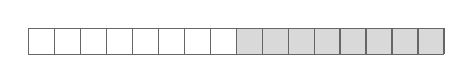
\begin{tikzpicture}[scale=0.33]
  % Grid lines
  \fill[black!15] (8cm,0) rectangle ++(8cm,1cm);
  \draw[step=1cm, black!60] (16,1) grid (0,0);
\end{tikzpicture} \onslide<9>{$r_1 = 0$}

\onslide<5->{
2) $x \text{ mod } 8 \geq 4$
\hspace{0.18cm}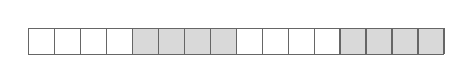
\begin{tikzpicture}[scale=0.33]
  % Grid lines
  \fill[black!15] (4cm,0) rectangle ++(4cm,1cm);
  \fill[black!15] (12cm,0) rectangle ++(4cm,1cm);
  \draw[step=1cm, black!60] (16,1) grid (0,0);
\end{tikzpicture} \onslide<9>{$r_2 = 1$}
}

\onslide<6->{
3) $x \text{ mod } 4 \geq 2$
\hspace{0.18cm}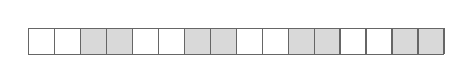
\begin{tikzpicture}[scale=0.33]
  % Grid lines
  \fill[black!15] (2cm,0) rectangle ++(2cm,1cm);
  \fill[black!15] (6cm,0) rectangle ++(2cm,1cm);
  \fill[black!15] (10cm,0) rectangle ++(2cm,1cm);
  \fill[black!15] (14cm,0) rectangle ++(2cm,1cm);
  \draw[step=1cm, black!60] (16,1) grid (0,0);
\end{tikzpicture} \onslide<9>{$r_3 = 1$}
}

\onslide<7->{
4) $x \text{ mod } 2 \geq 1$
\hspace{0.18cm}
\begin{tikzpicture}[scale=0.33]
  % Grid lines
  \fill[black!15] (1cm,0) rectangle ++(1cm,1cm);
  \fill[black!15] (3cm,0) rectangle ++(1cm,1cm);
  \fill[black!15] (5cm,0) rectangle ++(1cm,1cm);
  \fill[black!15] (7cm,0) rectangle ++(1cm,1cm);
  \fill[black!15] (9cm,0) rectangle ++(1cm,1cm);
  \fill[black!15] (11cm,0) rectangle ++(1cm,1cm);
  \fill[black!15] (13cm,0) rectangle ++(1cm,1cm);
  \fill[black!15] (15cm,0) rectangle ++(1cm,1cm);
  \draw[step=1cm, black!60] (16,1) grid (0,0);
\end{tikzpicture} \onslide<9>{$r_4 = 0$}
}\only<8>{\\[-0.4cm]
\centering
\begin{align*}
h(x \text{ mod } N \geq N/2) = - \log_2 \frac{1}{2} = 1 \text{ bit }
\end{align*}
}
\onslide<9>{\\[0.3cm]
\centering \Large
Necesitamos $\lceil \log_2 x\rceil$ bits para representar hasta el número $x$
}

\end{textblock}
}


\end{frame}


\begin{frame}[plain]
 \begin{textblock}{160}(0,4)
 \centering \LARGE Información en órdenes de magnitud\\
 \large Información de Shannon
\end{textblock}
\vspace{0.75cm}

\begin{textblock}{30}(5,30) \centering
 \ \normalsize Submarino: \\[0.2cm]

\begin{tikzpicture}[scale=0.33] \scriptsize
  \draw[step=1cm, black!60] (8,8) grid (0,0);
  \node at (-0.75,0.5) {1};
  \node at (-0.75, 1.5) {2};
  \foreach \x/\y in {-0.75/2.5} {\node at (\x, \y) {3};}
  \foreach \x/\y in {-0.75/3.5} {\node at (\x, \y) {4};}
  \foreach \x/\y in {-0.75/4.5} {\node at (\x, \y) {5};}
  \foreach \x/\y in {-0.75/5.5} {\node at (\x, \y) {6};}
  \foreach \x/\y in {-0.75/6.5} {\node at (\x, \y) {7};}
  \foreach \x/\y in {-0.75/7.5} {\node at (\x, \y) {8};}
  \node at (0.5,-0.75) {A};
  \node at (1.5,-0.75) {B};
  \node at (2.5,-0.75) {C};
  \node at (3.5,-0.75) {D};
  \node at (4.5,-0.75) {E};
  \node at (5.5,-0.75) {F};
  \node at (6.5,-0.75) {G};
  \node at (7.5,-0.75) {H};
  \only<2-3>{\draw[red, thick] (0.5cm, 0.5cm) circle [radius=0.4cm];}
  \only<4-6>{\node at (0.5,0.5) {x};}
  \only<5-6>{\node at (0.5,1.5) {x};}
  \only<5>{\draw[red, thick] (0.5cm, 1.5cm) circle [radius=0.4cm];}
  \only<7->{\foreach \x/\y in {
    0.5/0.5,1.5/0.5,2.5/0.5,3.5/0.5,
    0.5/1.5,1.5/1.5,2.5/1.5,3.5/1.5,
    0.5/2.5,1.5/2.5,2.5/2.5,3.5/2.5,
    0.5/3.5,1.5/3.5,2.5/3.5,3.5/3.5,
    0.5/4.5,1.5/4.5,2.5/4.5,3.5/4.5,
    0.5/5.5,1.5/5.5,2.5/5.5,3.5/5.5,
    0.5/6.5,1.5/6.5,2.5/6.5,3.5/6.5,
    0.5/7.5,1.5/7.5,2.5/7.5,3.5/7.5} {\node at (\x, \y) {x};} }
    \only<9->{\foreach \x/\y in {
    6.5/0.5,7.5/0.5,
    6.5/1.5,7.5/1.5,
    6.5/2.5,7.5/2.5,
    6.5/3.5,7.5/3.5,
    6.5/4.5,7.5/4.5,
    6.5/5.5,7.5/5.5,
    6.5/6.5,7.5/6.5,
    6.5/7.5,7.5/7.5} {\node at (\x, \y) {x};} }
    \only<10->{
      \fill[black!25, draw=black!60] (5cm,7cm) rectangle ++(1cm,1cm);
    }
    \only<10>{\draw[red, thick] (5.5cm, 7.5cm) circle [radius=0.4cm];}
\end{tikzpicture}
\end{textblock}

\only<2-3>{
\begin{textblock}{130}(43,20) \normalsize
\begin{flalign*}
& \onslide<3->{-\log_2} P(A1 = 1) = \only<2>{1/64}\only<3->{6 \text{ bits }} \\
&
&&
\end{flalign*}
\end{textblock}
}


\only<4->{
\begin{textblock}{130}(43,20) \normalsize
\begin{flalign*}
& -\log_2 P(A1 = 0) = \log_2 64/63 = 0.0227 \text{ bit } \\
\onslide<5->{& -\log_2 P(A2 = 0| A1 = 0) = \log_2 63/62} \onslide<6->{= 0.0230 \text{ bit } \\}
&&
\end{flalign*}
\end{textblock}
}


\only<7->{
\begin{textblock}{130}(43,38) \normalsize
\begin{flalign*}
& \log_2 64/63 + \log_2 63/62 + \dots + \log_2 33/32 \\
\only<8>{& \ \ \, 0.0227 \, \ \  +  \ \ \, 0.0230  \, \ \  + \dots + \ \, 0.0430 \ \ = 1.0 \text{ bit }}
\only<9->{& \log_2 32/31 + \log_2 31/30 + \dots + \log_2 17/16 \only<9>{= 2.0 \text{ bit }}\only<10->{+\underbrace{\log_2 16/1}_{4.0\text{ bit}} = 6.0 \text{ bit }} \\}
&&
\end{flalign*}
\end{textblock}
}

\only<11->{
\begin{textblock}{130}(28,64) \normalsize
\begin{flalign*}
& \phantom{\log_2 \frac{\cancel{64}}{\cancel{63}}} \log_2 \frac{64}{\only<11>{63}\only<12->{\cancel{63}}} + \log_2 \frac{\only<11>{63}\only<12->{\cancel{63}}}{\only<11-12>{62}\only<13->{\cancel{62}}} + \dots + \log_2 \frac{\only<11-12>{n+1}\only<13->{\cancel{n+1}}}{\only<11-12>{n}\only<13->{\cancel{n}}} + \log_2 \frac{\only<11-12>{n}\only<13->{\cancel{n}}}{1} \only<14->{= \log_2 \frac{64}{1} = 6.0 \text{ bit}}
&&
\end{flalign*}
\end{textblock}
}

\end{frame}

\begin{frame}[plain]
\begin{textblock}{160}(0,4)
\centering \LARGE Principio de no mentir \\
\large Máxima incertidumbre dada información disponible
\end{textblock}

\only<1-2>{
\begin{textblock}{160}(1,18) \centering \normalsize
\begin{flalign*}
P(\text{D}_{_T} = \{\overbrace{n_{s2}, n_{s3}}^{T}, \overbrace{n_{r1}, n_{r0}}^{T} \} \, | \, \text{M})^{1/T} &= \
P(s2|M)^{n_{s2}/T}  P(s3|M)^{n_{s3}/T} \, P(r1|M)^{n_{r1}/T} \, P(r0|M)^{n_{r0}/T}  \\
\underbrace{\log \ \ \lim_{T \rightarrow \infty} P(\text{D}|\text{M})^{1/T}}_{\hfrac{\text{\footnotesize Tasa de predicción}}{\text{\footnotesize en orden de magnitud}}} & = \ \  \sum_x \, p_{_{x}} \, \log p_{_{x}}  = -\underbrace{\textbf{Entropía}}_{\hfrac{\text{\footnotesize \phantom{p}Tasa de información}\phantom{p}}{\text{\footnotesize orden de magnitud}}}
&&
\end{flalign*}

\vspace{1cm}

\only<2>{
\Large Maximizar la entropía $ = \underbrace{\text{minimizar la tasa de predicción}}_{\text{Maximizar la \textbf{incertidumbre}}}$

}
\end{textblock}
}


\only<3->{
\begin{textblock}{45}(5,26) \centering \normalsize
Distribuciones de creencias{\footnotesize \\[-0.1cm] (por máxima entropía)}
\begin{flalign*}
\text{max } & - \int P(x) \log P(x) \, dx \\
\text{dado } & \int P(x)\,dx = 1 \\
              & \int f_k(x) P(x)\,dx = F_k \ \ \forall_k
&&
\end{flalign*}

\end{textblock}
}

\only<4->{
\begin{textblock}{110}(50,26) \centering
La familia exponencial \hspace{1cm} \normalsize
\begin{align*}
P(x|\theta) & = \frac{1}{Z(\theta)} h(x) \text{exp}(\theta^T \phi(x)) \\[0.2cm]
\onslide<4>{\text{Con:} & \\
& x\in \mathbb{X}^m \text{ hipótesis } \\
& \theta \in \mathbb{R}^d \text{ parámetros naturales } \\
& \phi(x) \in \mathbb{R}^d \text{ estadísticos suficientes } \\}
\end{align*}
\end{textblock}
}

\only<5>{
\begin{textblock}{110}(80,48) \small
$\bullet$ Uniforme$(x|a,b)$

$\bullet$ Bernoulli$(x|p)$

$\bullet$ Beta$(x|\alpha, \beta)$

$\bullet$ Geométrica$(x|p)$

$\bullet$ Multinomial$(x|p,n)$

$\bullet$ Hipergeométrica$(x|n,N,K)$

$\bullet$ Poisson$(x|\lambda)$

$\bullet$ Gaussiana$(x|\mu, \sigma^2)$

$\bullet$ \dots
\end{textblock}
}

\end{frame}

\begin{frame}[plain, fragile]
\begin{textblock}{160}(0,4)
\centering \LARGE Tasa de información \\
\large de los sistemas de comunicación
\end{textblock}

\only<1>{
\begin{textblock}{160}(0,26)
\centering
\tikz{

\node[det] (fuente) {};
\node[const, left=of fuente] (fx) {$f(x)$};
\node[const, above=of fuente] (n_fuente) {\scriptsize Fuente};
\node[const, right=of fuente, yshift=-0.35cm, xshift=0.05cm] (mensaje_enviado) {$\hfrac{\text{Realidad}}{\text{causal}}$};


\node[det, right=of fuente, xshift=0.6cm ] (transmisor) {};
\node[const, above=of transmisor] (n_transmisor) {\scriptsize Dimensión};
\node[const, right=of transmisor, yshift=-0.35cm, xshift=0.05cm] (senal_enviada) {$\hfrac{\text{Realidad}}{\text{causal}}$};

\node[const, right=of transmisor, xshift=1.4cm] (punto) {.};

\node[det, right=of transmisor, xshift=0.7cm, yshift=1cm] (perceptor) {};
\node[const, above=of perceptor] (n_perceptor) {\scriptsize Procedimiento A};

\node[det, right=of transmisor, xshift=0.7cm,yshift=-1cm] (perceptor2) {};
\node[const, below=of perceptor2] (n_perceptor2) {\scriptsize Procedimiento B};



\node[det, right=of perceptor, xshift=0.7cm,yshift=-1cm] (receptor) {};
\node[const, above=of receptor] (n_receptor) {\scriptsize Modelo};
\node[const, right=of receptor, yshift=-0.2cm, xshift=0.05cm] (mensaje_recibido) {\scriptsize Inferencia};

\node[const, left=of receptor, yshift=-0.45cm,xshift=-0.05cm] (senal_recibidaB) {\scriptsize Indicador B};
\node[const, left=of receptor, yshift=0.45cm,xshift=-0.05cm] (senal_recibidaA) {\scriptsize Indicador A};


\node[const, left=of receptor, xshift=-1.4cm, yshift=0.2cm] (punto2A) {.};
\node[const, left=of receptor, xshift=0.17cm, yshift=0.2cm] (punto2AR) {.};
\node[const, left=of receptor, xshift=-1.4cm, yshift=-0.2cm] (punto2B) {.};
\node[const, left=of receptor, xshift=0.17cm, yshift=-0.2cm] (punto2BR) {.};


\node[det, right=of receptor, xshift=0.6cm ] (destino) {};
\node[const, above=of destino] (n_destino) {\scriptsize Destino};

\node[const, right=of destino] (y) {$y_1$};


\node[invisible, above=of fuente, yshift=0.5cm] (ia) {};
\node[invisible, left=of fuente, xshift=-0.5cm] (il) {};
\node[invisible, right=of destino, xshift=0.5cm] (ir) {};


\edge {fuente} {transmisor};
\edge[-] {transmisor} {punto};
\edge {punto} {perceptor, perceptor2};
\edge[-] {perceptor} {punto2A};
\edge[-] {perceptor2} {punto2B};
\edge {punto2A} {punto2AR};
\edge {punto2B} {punto2BR};
\edge {receptor} {destino};

}

\vspace{1cm}

\Large \centering

Evaluar procedimientos alternativos.

\end{textblock}
}
\end{frame}

\begin{frame}[plain, fragile]
\begin{textblock}{160}(0,4)
\centering \LARGE Evaluación de test diagnóstico \\
\large Test rápido de chagas
\end{textblock}

\only<1-3>{
\begin{textblock}{160}(0,16)
\includegraphics[width=0.4\textwidth]{../../auxiliar/static/test_chagas.png}
\end{textblock}
}

\only<2-14>{
\begin{textblock}{100}(60,20) \normalsize
$P(\text{Diagnóstico}|\text{Estado})$ \\[0.3cm]

\begin{tabular}{|c|c|c|} \hline  \setlength\tabcolsep{0.4cm}
 & \hspace{0.1cm} D = Positivo \hspace{0.1cm} & \hspace{0.1cm} D = Negativo \hspace{0.1cm} \\ \hline
E = Verdadero & \only<2>{\textbf{Sensibilidad}}\only<3->{$s$} & \only<2>{1-Sensibilidad}\only<3->{$1-s$} \\ \hline
E = Falso     & \only<2>{1-Especificidad}\only<3->{$1-x$} & \only<2>{\textbf{Especificidad}}\only<3->{$x$} \\ \hline
  \end{tabular}
\only<4->{
\begin{flalign*}
& p \sim \text{Beta}(\alpha, \beta) \\
\only<5-6>{
  & q = p \, s + (1-p) \, (1-x) \\
}
\only<6>{
  &r = (\underbrace{n_0}_{-}, \underbrace{n_1}_{+})  \sim \text{ Binomial}(q,N) \\
}
\only<7->{
  &r = (\underbrace{n_0}_{--}, \underbrace{n_1}_{-+}, \underbrace{n_2}_{+-}, \underbrace{n_3}_{++}) \sim \text{ Multinomial}(q,N) \\
}
\only<8->{
  & q = (\ q_0\ , \ q_1 \ , \ q_2, \ q_3 \ )\\
}
\only<9-11>{
  & \ \ q_0 = p \, (1-s_a) \, (1-s_b) + (1-p) \, x_a \, x_b \\
}
\only<10-11>{
  & \ \ q_1 = p \, (1-s_a) \, s_b + (1-p) \, x_a \, (1-x_b) \\
}
\only<11>{
  & \ \ q_2 = \dots \\
}
&&
\end{flalign*}
}
\end{textblock}
}

\only<12>{
\begin{textblock}{100}(50,73) \centering
Problema no identificable \\ \normalsize
5 hipótesis ($p,s_a,x_a,s_b,x_b$) y 3 datos ($n_0, n_1, n_2$)
\end{textblock}
}
\only<14>{
\begin{textblock}{120}(40,73) \centering
Problema identificable \\ \small
6 hipótesis ($p_A,p_B,s_a,x_a,s_b,x_b$) y 6 datos ($r_A, r_B$)
\end{textblock}
}


\only<4->{
\begin{textblock}{160}(0,14)
\scalebox{0.85}{
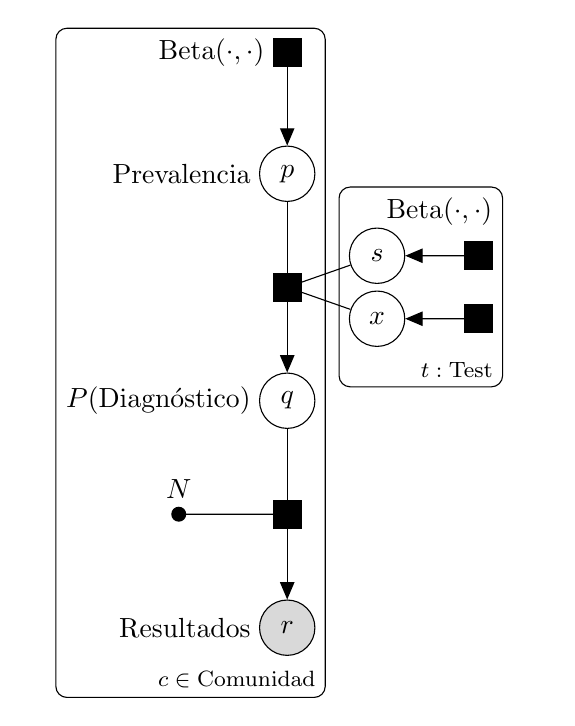
\begin{tikzpicture}[scale=0.33]
    \node[factor] (fp) {};
    \node[const, left=of fp] (nfp) {Beta$(\cdot,\cdot)$};
    \node[latent, below=of fp] (p) {$p$};
    \node[const, left=of p] (np) {Prevalencia};
    \onslide<5->{
      \node[factor, below=of p, yshift=0.1cm] (fq) {};
      \node[latent, below=of fq, yshift=0.1cm] (q) {$q$};
      \node[latent, right=of fq, xshift=-0.4cm, yshift=0.4cm] (s) {$s$};
      \node[latent, right=of fq, xshift=-0.4cm, yshift=-0.4cm] (x) {$x$};
      \node[factor, right=of s, xshift=-0.25cm] (fs) {};
      \node[factor, right=of x, xshift=-0.25cm] (fx) {};
      \node[const, above=of fs, xshift=-0.5cm, yshift=0.1cm] (ps) {Beta$(\cdot,\cdot)$};
      \node[const, left=of q] (nq) {$P(\text{Diagnóstico})$};
    }
    \onslide<6->{
      \node[factor, below=of q, yshift=0.1cm] (fr) {};
      \node[latent, below=of fr, fill=black!15, yshift=0.1cm] (r) {$r$};
      \node[const, left=of r] (nr) {Resultados};
      \node[accion, left=of fr, xshift=-0.7cm] (N) {};
      \node[const, above=of N] (nN) {$N$};
    }

    \edge {fp} {p};
    \onslide<5->{
      \edge[-] {p,s,x} {fq};
      \edge {fq} {q};
      \edge {fs} {s};
      \edge {fx} {x};
    }
    \onslide<6->{
      \edge[-] {q, N} {fr};
      \edge {fr} {r};
    }

    \onslide<7->{\plate {test} {(s)(x)(ps)} {$t:\text{Test}$};}
    \onslide<13->{\plate {poblacion} {(fp)(p)(q)(r)(N)(nq)} {$c \in \text{Comunidad}$};}

    \node[invisible, left=of fp, xshift=-3cm] (il) {};
    \node[invisible, right=of fp, xshift=3cm] (i3) {};
\end{tikzpicture}
}
\end{textblock}
}

\end{frame}



\begin{frame}[plain, fragile]
\begin{textblock}{160}(0,4)
\centering \LARGE Evaluación de test diagnóstico
\end{textblock}


\begin{textblock}{160}(0,14)
\scalebox{0.85}{
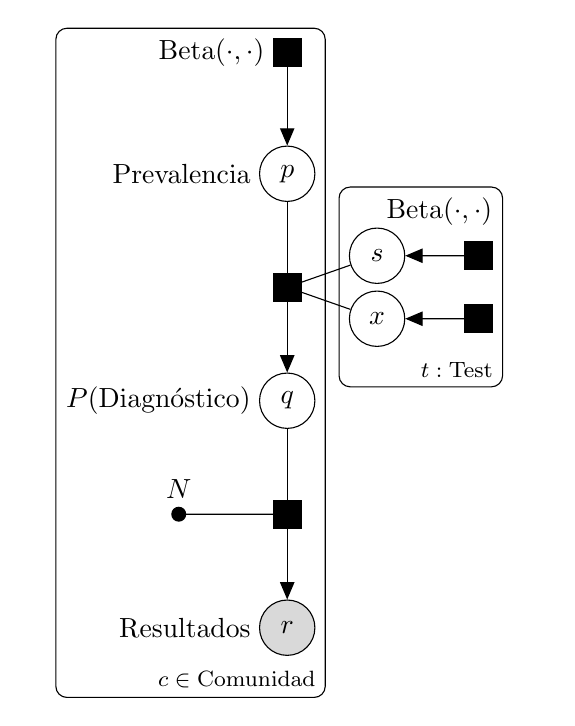
\begin{tikzpicture}[scale=0.33]
    \node[factor] (fp) {};
    \node[const, left=of fp] (nfp) {Beta$(\cdot,\cdot)$};
    \node[latent, below=of fp] (p) {$p$};
    \node[const, left=of p] (np) {Prevalencia};
      \node[factor, below=of p, yshift=0.1cm] (fq) {};
      \node[latent, below=of fq, yshift=0.1cm] (q) {$q$};

      \node[latent, right=of fq, xshift=-0.4cm, yshift=0.4cm] (s) {$s$};
      \node[latent, right=of fq, xshift=-0.4cm, yshift=-0.4cm] (x) {$x$};
      \node[factor, right=of s, xshift=-0.25cm] (fs) {};
      \node[factor, right=of x, xshift=-0.25cm] (fx) {};
      \node[const, above=of fs, xshift=-0.5cm, yshift=0.1cm] (ps) {Beta$(\cdot,\cdot)$};
      \node[const, left=of q] (nq) {$P(\text{Diagnóstico})$};
      \node[factor, below=of q, yshift=0.1cm] (fr) {};
      \node[latent, below=of fr, fill=black!15, yshift=0.1cm] (r) {$r$};
      \node[const, left=of r] (nr) {Resultados};
      \node[accion, left=of fr, xshift=-0.7cm] (N) {};
      \node[const, above=of N] (nN) {$N$};

    \edge {fp} {p};
      \edge[-] {p,s,x} {fq};
      \edge {fs} {s};
      \edge {fx} {x};
      \edge {fq} {q};
      \edge[-] {q, N} {fr};
      \edge {fr} {r};

    \plate {test} {(s)(x)(ps)} {$t:\text{Test}$};
    \plate {poblacion} {(fp)(p)(q)(r)(N)(nq)} {$c \in \text{Comunidad}$};

    \node[invisible, left=of fp, xshift=-3cm] (il) {};
    \node[invisible, right=of fp, xshift=3cm] (i3) {};
\end{tikzpicture}
}
\end{textblock}


\begin{textblock}{100}(57,8)
\begin{lstlisting}[backgroundcolor=\color{black!10}]
modelo <- "model{
  s[1] ~ dbeta(1, 1)
  s[2] ~ dbeta(1, 1)
  x[1] ~ dbeta(1, 1)
  x[2] ~ dbeta(1, 1)

  for(c in 1:Comunidades){
    p[c] ~ dbeta(1, 1)

    q[1,c] <- p[c]*(1-s[1])*(1-s[2]) + (1-p[c])*x[1]*x[2]
    q[2,c] <- p[c]*(1-s[1])*s[2] + (1-p[c])*x[1]*(1-x[2])
    q[3,c] <- p[c]*s[1]*(1-s[2]) + (1-p[c])*(1-x[1])*x[2]
    q[4,c] <- p[c]*s[1]*s[2] + (1-p[c])*(1-x[1])*(1-x[2])

    r[1:4, c] ~ dmulti(q[1:4, c], N[c])
  }
  #data# r, N, Comunidades
  #monitor# p, s, x
  #inits# p, s, x
}"
\end{lstlisting}
\end{textblock}

\end{frame}



\begin{frame}[plain, fragile]
\begin{textblock}{160}(0,4)
\centering \LARGE Evaluación de test diagnóstico
\end{textblock}


\begin{textblock}{160}(0,14)
\scalebox{0.85}{
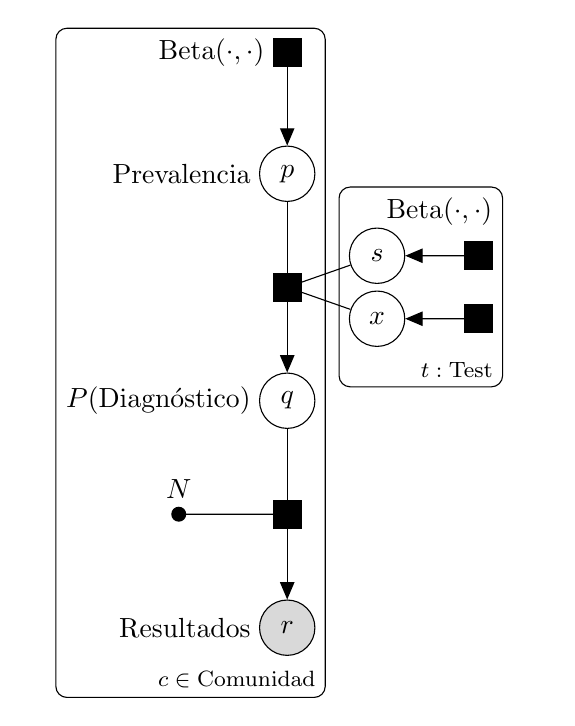
\begin{tikzpicture}[scale=0.33]
    \node[factor] (fp) {};
    \node[const, left=of fp] (nfp) {Beta$(\cdot,\cdot)$};
    \node[latent, below=of fp] (p) {$p$};
    \node[const, left=of p] (np) {Prevalencia};
      \node[factor, below=of p, yshift=0.1cm] (fq) {};
      \node[latent, below=of fq, yshift=0.1cm] (q) {$q$};

      \node[latent, right=of fq, xshift=-0.4cm, yshift=0.4cm] (s) {$s$};
      \node[latent, right=of fq, xshift=-0.4cm, yshift=-0.4cm] (x) {$x$};
      \node[factor, right=of s, xshift=-0.25cm] (fs) {};
      \node[factor, right=of x, xshift=-0.25cm] (fx) {};
      \node[const, above=of fs, xshift=-0.5cm, yshift=0.1cm] (ps) {Beta$(\cdot,\cdot)$};
      \node[const, left=of q] (nq) {$P(\text{Diagnóstico})$};
      \node[factor, below=of q, yshift=0.1cm] (fr) {};
      \node[latent, below=of fr, fill=black!15, yshift=0.1cm] (r) {$r$};
      \node[const, left=of r] (nr) {Resultados};
      \node[accion, left=of fr, xshift=-0.7cm] (N) {};
      \node[const, above=of N] (nN) {$N$};

    \edge {fp} {p};
      \edge[-] {p,s,x} {fq};
      \edge {fs} {s};
      \edge {fx} {x};
      \edge {fq} {q};
      \edge[-] {q, N} {fr};
      \edge {fr} {r};

    \plate {test} {(s)(x)(ps)} {$t:\text{Test}$};
    \plate {poblacion} {(fp)(p)(q)(r)(N)(nq)} {$c \in \text{Comunidad}$};

    \node[invisible, left=of fp, xshift=-3cm] (il) {};
    \node[invisible, right=of fp, xshift=3cm] (i3) {};
\end{tikzpicture}
}
\end{textblock}


\begin{textblock}{100}(57,8)
\begin{lstlisting}[backgroundcolor=\color{black!10}]
library("runjags") # JAGS: Just Another Gibbs Sampler

p = c(0, 0.15, 0.3, 0.45, 0.7) # REALIDAD
sensitivity = c(0.9, 0.6)
specificity = c(0.95, 0.9)

r <- matrix(nrow=4, ncol=length(p)) # DATA (simulada)
r[,1] <- c(839, 104, 44, 7)
r[,2] <- c(754, 92,  85, 92)
r[,3] <- c(598, 99, 134, 151)
r[,4] <- c(503, 75, 187, 240)
r[,5] <- c(275, 61, 287, 373)
N <- apply(r, MARGIN=2, FUN=sum); Comunidades = 5

s <- list(chain1=c(0.5,0.99), chain2=c(0.99,0.5)) # INITS
x <- list(chain1=c(0.5,0.99), chain2=c(0.99,0.5))
p <- list(chain1=c(0.1, 0.1, 0.1, 0.9, 0.9), chain2=c(0.9, 0.9, 0.9, 0.1, 0.1))

results <- run.jags(modelo, n.chains=2)
\end{lstlisting}
\end{textblock}

\end{frame}



\begin{frame}[plain, fragile]
\begin{textblock}{160}(0,4)
\centering \LARGE Evaluación de test diagnóstico
\end{textblock}


\begin{textblock}{160}(0,14)
\scalebox{0.85}{
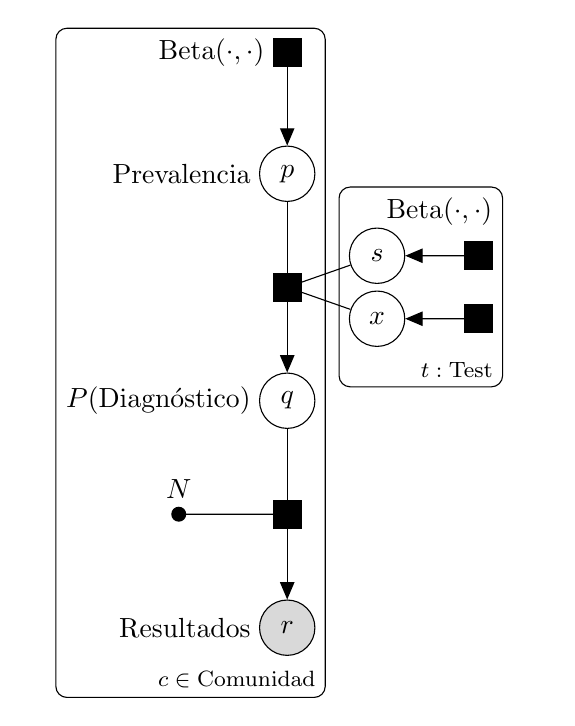
\begin{tikzpicture}[scale=0.33]
    \node[factor] (fp) {};
    \node[const, left=of fp] (nfp) {Beta$(\cdot,\cdot)$};
    \node[latent, below=of fp] (p) {$p$};
    \node[const, left=of p] (np) {Prevalencia};
      \node[factor, below=of p, yshift=0.1cm] (fq) {};
      \node[latent, below=of fq, yshift=0.1cm] (q) {$q$};

      \node[latent, right=of fq, xshift=-0.4cm, yshift=0.4cm] (s) {$s$};
      \node[latent, right=of fq, xshift=-0.4cm, yshift=-0.4cm] (x) {$x$};
      \node[factor, right=of s, xshift=-0.25cm] (fs) {};
      \node[factor, right=of x, xshift=-0.25cm] (fx) {};
      \node[const, above=of fs, xshift=-0.5cm, yshift=0.1cm] (ps) {Beta$(\cdot,\cdot)$};
      \node[const, left=of q] (nq) {$P(\text{Diagnóstico})$};
      \node[factor, below=of q, yshift=0.1cm] (fr) {};
      \node[latent, below=of fr, fill=black!15, yshift=0.1cm] (r) {$r$};
      \node[const, left=of r] (nr) {Resultados};
      \node[accion, left=of fr, xshift=-0.7cm] (N) {};
      \node[const, above=of N] (nN) {$N$};

    \edge {fp} {p};
      \edge[-] {p,s,x} {fq};
      \edge {fs} {s};
      \edge {fx} {x};
      \edge {fq} {q};
      \edge[-] {q, N} {fr};
      \edge {fr} {r};

    \plate {test} {(s)(x)(ps)} {$t:\text{Test}$};
    \plate {poblacion} {(fp)(p)(q)(r)(N)(nq)} {$c \in \text{Comunidad}$};

    \node[invisible, left=of fp, xshift=-3cm] (il) {};
    \node[invisible, right=of fp, xshift=3cm] (i3) {};
\end{tikzpicture}
}
\end{textblock}


\begin{textblock}{100}(57,8)
\begin{lstlisting}[backgroundcolor=\color{black!10}]
     Lower95 Median  Upper95    #Real
p[1] 6e-07   0.0071  0.0184     #0.00
p[2] 0.1213  0.1501  0.1792     #0.15
p[3] 0.2478  0.2829  0.3207     #0.30
p[4] 0.3922  0.4324  0.4718     #0.45
p[5] 0.6573  0.7016  0.7428     #0.70
s[1] 0.8822  0.9233  0.9646     #0.95
s[2] 0.5556  0.5829  0.6129     #0.60
x[1] 0.9429  0.9566  0.9705     #0.95
x[2] 0.8755  0.8897  0.9034     #0.90
     SSeff  AC.10    psrf
p[1]  5575 0.02143  1.0000
p[2]  6162 0.03274  1.0002
p[3]  5323 0.01990  1.0000
p[4]  4992 0.04256  0.9999
p[5]  3730 0.04781  1.0004
s[1]  2742 0.08044  1.0009
s[2]  7065 0.01934  1.0002
x[1]  4558 0.04616  1.0007
x[2]  4260 0.04574  1.0001
\end{lstlisting}
\end{textblock}

\end{frame}

\begin{frame}[plain, fragile]
\begin{textblock}{160}(0,4)
\centering \LARGE Tasa de información \\
\large de los sistemas de comunicación
\end{textblock}

\only<1>{
\begin{textblock}{160}(0,26)
\centering
\tikz{

\node[det] (fuente) {};
\node[const, left=of fuente] (fx) {$f(x)$};
\node[const, above=of fuente] (n_fuente) {\scriptsize Fuente};
\node[const, right=of fuente, yshift=-0.35cm, xshift=0.05cm] (mensaje_enviado) {$\hfrac{\text{Realidad}}{\text{causal}}$};


\node[det, right=of fuente, xshift=0.6cm ] (transmisor) {};
\node[const, above=of transmisor] (n_transmisor) {\scriptsize Dimensión};
\node[const, right=of transmisor, yshift=-0.35cm, xshift=0.05cm] (senal_enviada) {$\hfrac{\text{Realidad}}{\text{causal}}$};

\node[const, right=of transmisor, xshift=1.4cm] (punto) {.};

\node[det, right=of transmisor, xshift=0.7cm, yshift=1cm] (perceptor) {};
\node[const, above=of perceptor] (n_perceptor) {\scriptsize Procedimiento A};

\node[det, right=of transmisor, xshift=0.7cm,yshift=-1cm] (perceptor2) {};
\node[const, below=of perceptor2] (n_perceptor2) {\scriptsize Procedimiento B};



\node[det, right=of perceptor, xshift=0.7cm,yshift=-1cm] (receptor) {};
\node[const, above=of receptor] (n_receptor) {\scriptsize Modelo};
\node[const, right=of receptor, yshift=-0.2cm, xshift=0.05cm] (mensaje_recibido) {\scriptsize Inferencia};

\node[const, left=of receptor, yshift=-0.45cm,xshift=-0.05cm] (senal_recibidaB) {\scriptsize Indicador B};
\node[const, left=of receptor, yshift=0.45cm,xshift=-0.05cm] (senal_recibidaA) {\scriptsize Indicador A};


\node[const, left=of receptor, xshift=-1.4cm, yshift=0.2cm] (punto2A) {.};
\node[const, left=of receptor, xshift=0.17cm, yshift=0.2cm] (punto2AR) {.};
\node[const, left=of receptor, xshift=-1.4cm, yshift=-0.2cm] (punto2B) {.};
\node[const, left=of receptor, xshift=0.17cm, yshift=-0.2cm] (punto2BR) {.};


\node[det, right=of receptor, xshift=0.6cm ] (destino) {};
\node[const, above=of destino] (n_destino) {\scriptsize Destino};

\node[const, right=of destino] (y) {$y_1$};


\node[invisible, above=of fuente, yshift=0.5cm] (ia) {};
\node[invisible, left=of fuente, xshift=-0.5cm] (il) {};
\node[invisible, right=of destino, xshift=0.5cm] (ir) {};


\edge {fuente} {transmisor};
\edge[-] {transmisor} {punto};
\edge {punto} {perceptor, perceptor2};
\edge[-] {perceptor} {punto2A};
\edge[-] {perceptor2} {punto2B};
\edge {punto2A} {punto2AR};
\edge {punto2B} {punto2BR};
\edge {receptor} {destino};

}

\vspace{1cm}

\Large \centering

¿Con qué procedimiento nos quedamos?

\end{textblock}
}
\end{frame}



\begin{frame}[plain,noframenumbering]
\centering \vspace{0.5cm}
\includegraphics[width=1\textwidth]{../../auxiliar/static/BP.png}
\end{frame}





%
% \begin{frame}[plain]
% \begin{textblock}{96}(0,6.5)\centering
% {\transparent{0.9}\includegraphics[width=0.8\textwidth]{../../auxiliar/static/inti.png}}
% \end{textblock}
%
% \begin{textblock}{160}(96,5.5)
% \includegraphics[width=0.35\textwidth]{../../auxiliar/static/pachacuteckoricancha}
% \end{textblock}
% \end{frame}





\end{document}



